%!TEX program = xelatex
\documentclass[fleqn,10pt]{olplainarticle}
% Use option lineno for line numbers 
\usepackage{xcolor}
\usepackage{framed}
\usepackage{hyperref}
\colorlet{darkblue}{blue!40!black}
\hypersetup{
    colorlinks=true,
    linkcolor=blue,
    filecolor=magenta,
    urlcolor=cyan,
    citecolor=darkblue
}
\urlstyle{same}

\usepackage{imakeidx}
\makeindex

\usepackage{xspace}
\usepackage[utf8]{inputenc}
\usepackage{fontspec}
% This section makes Fira work.
\setmonofont{Fira Code}[
  Contextuals=Alternate  % Activate the calt feature
]

\makeatletter
\def\verbatim@nolig@list{}%
\makeatother

\usepackage{listings}
\usepackage{lstfiracode}
\usepackage{url}


% For natbib, \citet for textual, \citep for parenthetical,
% \citeauthor and \citeyear.
\newenvironment{callout}
{
\begin{figure}
\begin{center}
\begin{minipage}{0.9\textwidth}
\begin{framed}
}
{
\end{framed}
\end{minipage}
\end{center}
\end{figure}
}
\newcommand{\rlang}{\textsc{r}\xspace}
\newcommand{\cpp}{\textsc{c}++\xspace}
\newcommand{\cpu}{\textsc{cpu}\xspace}
\newcommand{\nan}{\textsc{NaN}\xspace}
\newcommand{\ieee}{\textsc{ieee}\xspace}
\newcommand{\aside}[1]{\textcolor{red}{#1}}

\title{Testing Scientific Code}

\author[1]{Andrew Dolgert}
\affil[1]{IHME, University of Washington}

\keywords{software testing, unit testing, scientific software}

\begin{document}
\lstset{
  style=FiraCodeStyle,
  basicstyle=\footnotesize\ttfamily,
  %backgroundcolor=\color{green!20}
  }

\begin{abstract}
When we write code to do science, even though we have purposefully
chosen each step of the code, we may not know what the exact result should be.
Not having an exact right answer makes unit testing both complicated and
critical to trusting the scientific results. This article doesn't show how
to set up unit testing in \rlang, Python, or Julia. It doesn't cover numerical
analysis. It shows how to put boundaries on the behavior of mathematical
code. Some techniques are adaptations of traditional unit testing methods
and others are particular to testing scientific code.
\end{abstract}

% Audience:
% a) researchers who write code but don't know how to turn notebooks
%    into unit tests.
% b) software engineers who implement code but aren't sure how to handle
%    tests of squirrelly math.

% Intention:
% Sleuthing to reveal how mathematical expectations become test assertions.
% Literature says research code has an "oracle problem."
% I don't like that term. So what if we don't know the exact number
% a function can produce? All unit testing, mathematical or otherwise
% is about testing whether expectations are met, and those can
% be hard to define. We always have some expectations
% about how new research code will behave. The challenge is to
% a) understand what our expectations are and b) express those
% expectations in unit tests in c) a way that reduces risk.

% Principles
%
% 1. No need to highlight arcane names (metamorphic, predicate).
% 2. Use "I" and "We".
% 3. Don't need to cover everything. (mutation testing is out).

% Major sections
% 1. Reading for risk
% 2. Parallel implementation
% 3. Statistics for tests
% 4. Deterministic repeated measures
% 5. Methods and motives, the process in context

% finite state machine structured testing

% From Mike Richards
% 2. Focus on moving up and down the stack, not between scientist and developer.
% You don't need to tell them everything about the subject.
% Alec contributed Pearson
% James presses about the audience and software vs. math.

% TODO
% Missing: fault localization, model-based testing
% add simple stats tests from the intro modern stats book
% add figures to explain pearson coefficient
% explain mantissa and exponent.
% add more symmetry examples.
% show path analysis and flow analysis as figures.
% Take a failing test and reduce the input until you have
% a smallest failing test. Very helpful for identifying failures.

% High level tests will test more.
%                  will make it harder to find a fault.
%                  will make it harder to identify a _failure._


\flushbottom
\maketitle
\thispagestyle{empty}

\tableofcontents
\section{Introduction}\label{sec:introduction}

% In most code, you expect a value. For scientific code, your
% expectations are properties of the code or in relation to
% previous work. It's about discovering expectations.

The code for a scientific application, laid out across a monitor,
will have plenty of functions that look like those of any other application.
It will parse command-line flags, parse input files, and maybe even have
an event loop. Some portion, however, will look entirely different. It
may be laden with long equations, or it may be integer manipulation or
graphs, but the functions that do this work are complex, and they carry risk.

The complexity of those scientific functions is necessary
in order to model some feature of the world. Their math, whether mundane
or arcane, makes it difficult to use traditional unit tests to address
the risk of failure in these functions. When a model is supposed to represent
a subtle behavior of the world, testing that its output is correct feels
like an existential assertion.

However, scientific models, and the functions that comprise them,
always have behavior we can discover, characterize, and assert in a unit
test. Some of that behavior is approximate and some exact.
It's this mathematical behavior that is our first concern for testing.
It's called functional testing, when we look for faults in the code
that would lead to failures when the code runs. We exclude, here,
questions of testing how long a function runs, how much memory it uses,
whether it's secure, or whether it's usable.

I met a man, at dinner at a wedding, who told me he quit his
job as \textsc{ceo} of a printer company in order to lead
the support division. He said the company was going downhill,
and there was no better way to find out why than to hear from
the customer about how their product failed.
For scientific code that supports research, it can be hard to
know when it's right or wrong, and unit testing is the
support division.

Even with this scope, of whether the function will, in the future,
give the right answer, it will become clear that, as complex as
code looks on a monitor, the work to reassure ourselves that it lacks
faults, that there is no character out of place, would be terribly more
work than to write the function. If each part of a scientific application
had an exhaustive suite of tests, it would become brittle to change,
the opposite of a tool for research.

The code we test has a topography of risk. Some of it is measurable,
as a number of if--then statements or a count of equation terms.
Some of it is a landscape of doubt, that these lines of code are
doing their job or that that language idiom is properly-written.
When a function fails to read a file, and it quits, that's less
a problem than a function that reads a file incorrectly and gives
a wrong result.

Assuming we've read a good unit testing book like \cite{jorgensen2013},
and that we can figure out, elsewhere, the idiosyncracies of a
particular language or testing framework,
let's assess here the risks that are unigue to scientific code.
Let's look at how the tools we already know can address those risks
and how some new tools might help when the stakes are high.



\section{When a fault is a problem}

Debugging code can take longer than writing it. You can see
a wrong answer and spend hours trying to figure out where the
calculation went wrong, in what function, in what data structure,
at what assignment statement.
Writing unit tests is like debugging code before you know
where the bugs are.

We prepare to test code by walking backwards, starting with
what we consider a problem. For this work, we want to find
ways the code will stop prematurely (or never stop)
and ways it will give a wrong answer masquerading as a right one.

Failures are evidence something went wrong. Since our main goal
is scientific correctness, we classify failures on two axes,
whether they are recoverable and how long it takes to discover
the failure. Some algorithms are allowed to fail for certain
input values, and we can recover by running a different, acceptable
algorithm. Failures can be immediate exceptions that provide
debugging information or abnormal termination that quits with
only a single error code, but they
could be \nan{}s that silently propagate through code. They
could be loops that don't terminate, so you wait hours to find
the problem.

How your scientific application handles failures, and how you
rank their severity, varies by application, as we can see from
a few examples. If a software application has a menu of operations
to perform, and one menu item incurs a fault, which creates an exception,
then maybe the user sees an error message. That's not intended, but
it means this one operation won't work on this data.
If the scientific application is part of a large pipeline of
work, and a fault creates a result that is out-of-bounds because
it is negative or \textsc{NaN}, then that could be \textsc{ok}
if there is a backup calculation that is more likely to succeed.
In most cases, if I'm doing science, my main worry is when a
fault \emph{doesn't lead to failure.} It's numbers that are
significantly different from the correct value but not obviously
wrong. It's faults without failures.

Failures come from defects in the code, which we call \emph{faults,}
and we classify these so that we know which are most important
to our task. The ODC classifies types of defects, in order to understand
how different types affect code across its development time.
\begin{itemize}
    \item \emph{Algorithm}---These are correctness problems
    that can be fixed within a function or local data structure.
    This includes both whether an equation is correct and whether
    a loop has an off-by-one error.

    \item \emph{Assignment}---These are incorrect initialization
    of control blocks or data structures.

    \item \emph{Checking}---Program logic around loop conditions
    and branching statements. This is about a wrong if--then. A mistaken condition can mean that
    the result would be correct for a different set of parameters.

    \item \emph{Interface}---Defects when calling other components
    or functions. This includes parameter lists.

    \item \emph{Functional}---This doesn't mean that defects are
    in functions. It means these are errors that require redesign
    of the code. It can mean moving code among functions, changing
    important data structures, or redesigning objects.

    \item \emph{Documentation}---Whether it's published documentation,
    code documentation, or maintenance notes, there can be
    correctness errors here.
\end{itemize}
Scientific equations are in the algorithm category, so that category
is the most immediate threat to correctness, but the
ODC paper observed that teams find algorithm defects early in the
development process. Meanwhile, faults in assignment and checking were
found later in the development process. A fault in checking would
mean an incorrect branch in the code. Even if the algorithm is
correct, the answer from the code would be inappropriate, so these
are no less wrong.

I read a story in the observations of the ODC paper. It says
that we first focus on the core math, and it has errors, but we
gradually work those out. Meanwhile, we build software around that
core math, and that software has features and options that multiply
algorithmic complexity and thus multiply problems.

Between these two kinds of errors, the algorithmic versus the
checking and assignment, there is difference in how they fail.
If an equation has a misplaced parenthesis or incorrect exponent,
it is more likely to return a number without raising an exception.
On the other hand, an off-by-one error in a loop, when it fails,
is more likely to create an out-of-bounds memory error. This visible
failure is a real problem in production code, but it is far
less insidious than a silent fault in the equation.

There's another classification scheme for faults that asks
where they happen, in what part of the code. For scientific computing,
we can use a traditional model of high-performance computing
to break the \emph{where} into a few pieces.
\begin{itemize}
    \item \emph{Parameter handling}---Faults interpreting input parameters.
    There is often an early step to turn the parameters a user specifies
    into an internal form that the algorithms need.

    \item \emph{Input/Output}---Faults when reading and writing
    data from/to any other component.

    \item \emph{Code movement}---The work to move data from input
    to the right data structure for an optimized algorithm. The work
    to take data out of one data structure and put it into another one.

    \item \emph{Algorithm}---Faults in what we consider the main
    computation. We tend to write code that centers on one
    or more algorithms.

    \item \emph{Visualization}---This is any output for the user. It
    can be in a window or graphs on disk. We separate this from the
    data input and output because it often has its own set of
    algorithms which can be as complicated as any other part of the code.
\end{itemize}
These different parts of the code tend to have different maturity levels
and different kinds of risks. They develop differently over time.
For instance, visualization algorithms can come pre-packaged, so that
most of the work is setting up the data and checking that it is valid
for the visualization method. For visualization, the failure may look
like a divide-by-zero, but the fault is more often input data that
is in error.

Code movement tends to have checking- and assignment-type errors,
while algorithm code tends to have, well, algorithm-type errors.
This points to a principle for how to group code.
\emph{Code Complete} gives seven types of cohesion that encourage
grouping code together~\citep{mcconnell2004code}. We can add to that list. We should group
code that needs similar kinds of unit testing because it poses
similar kinds of risk. Here, that means we would do complete
path testing on parameter handling. We might test random samples
of data structures for code movement portions.

We use unit tests to look for faults, but unit tests observe
failures. We can test less, and test better, by understanding
how to read code so that we see cause and effect.


\section{Path and data flow}

My first assignment in high school chemistry was a six-inch square
black box on my desk. Inside the box was some cardboard structure
and a single marble. I had to make a sketch of the hidden cardboard
structure by turning the box and feeling the weight of the marble
and as it moved. Even if I couldn't see inside the box, I
understood how a marble would balance, roll, and drop.

A unit test sets parameters on a function and checks its result.
I might get to read the code I'm testing (clear-box testing),
or not (black-box testing). In either case, I need a feel for
the physics of how each probing parameter might affect the
function's return value. Analyzing cause and effect in code
helps us read it. There are only three was we find problems
in code. We read it during code reviews, we test it, or we run it on
real world problems. The first two rely on reading code well,
and the third is the definition of failure.

\subsection{Code paths}\label{sec:code-paths}

If I look at the code in a function, it typically has
some if--thens, some while--loops, some for--loops. These
control structures determine which lines of the code do
or don't get executed, depending on the input parameters.
When we analyze code according to its control structures,
it's called path analysis.

Let's take a running average as an example. This code
averages values over several days, and it will take an
average of the last several days, the next several days,
or in-between. It's implemented without using \lstinline|numpy|,
as an example. Look for control structures in this function.

\begin{lstlisting}[language=Python,numbers=left]
def running_average(x, duration, orientation, fill):
    offsets = {
        "past": 1 - duration,
        "future": 0,
        "midpoint": 1 - ((duration + 1) // 2)
        }
    offset_in_window = offsets[orientation]

    result = x[0:len(x)]
    if fill:
        filled = x[:1] * (duration - 1) + x + x[-1:] * (duration - 1)
        offset_in_window += duration - 1
        for i in range(0, len(x)):
            a, b = [i + offset_in_window, i + duration + offset_in_window]
            result[i] = sum(filled[a:b]) / duration
    else:
        for i in range(0, len(x)):
            a, b = [i + offset_in_window, i + duration + offset_in_window]
            left = max(a, 0)
            right = min(b, len(x))
            result[i] = sum(x[left:right]) / (right - left)
    return result
\end{lstlisting}

\noindent{}If \lstinline|fill=True|, the lines 11--15 are run.
If it's false, lines 17--21 are run. We can further subdivide
these two blocks by observing that, if the length of \lstinline|x|
is 0, then the for--loop won't run. Therefore, that's a separate
block too. The blocks above are
\begin{enumerate}
    \item Lines 2--10, Set offsets
    \item Lines 11-13, Create filled array
    \item Lines 13--15, For--loop over filled array
    \item Line 17, Without filling
    \item Lines 17--21, For--loop over array
    \item Line 22,
\end{enumerate}

There are four paths, which depend on \lstinline|fill|
and \lstinline|len(x) > 0|.
\begin{itemize}
    \item 1, 2, 3, 6
    \item 1, 2, 6
    \item 1, 4, 5, 6
    \item 1, 4, 6
\end{itemize}
Two of them are much less likely. You can either decide that
they are less important because they are less likely, or
you can decide that they are important to test separately
because other parts of the tests will cover the more common
paths.

Not every if--then is a separate path. Consider a case where
the same option is used twice.

\begin{lstlisting}[language=Python,numbers=left]
def sample(x, option = false):
    if option:
        k = 3
    else:
        k = 2
    y = k * x
    if option:
        z = [abs[m] for m in y]
    else:
        z = y
    return z
\end{lstlisting}

\noindent{}There are two if--thens, which would lead to four different
paths, except that they use the same condition. Depending on
how complicated the condition is, it may not be obvious that
the paths are related to each other.

Path testing is an approximation to the number of different
ways to call a function. Looking at the code line-by-line,
we can see finer branches in how a function handles inputs.
Branch points are conditions that depend on input values
but don't change which lines of code are run. For example,
data frames are built to enable easy branch points.
\begin{lstlisting}
under30 <- individuals_df[individuals_df$age < 30, ]
\end{lstlisting}
It isn't an if--then, but data above and below 30 will take
different paths through the code. Data frames are built
to handle complicated inputs, so they are built to create
complicated testing problems.

Path testing is a way to get a clear view of
the code, but it's just one model for how to read code.

\subsection{Data flow}
predicate-use (P-use) versue C-use.

Let's look at another piece of code, this one to integrate
a differential equation.
\begin{lstlisting}[numbers=left]
function explicit_euler_riemann(mu, beta, p0, h, t0, t1, a0, a1)
    a = a0:h:a1
    t = t0:h:t1
    m = length(a)
    n = length(t)

    u = zeros(h, m, n)
    u[:, 1] = p0(a, t0)

    for i in 1:(n - 1)
        u[:, i + 1] = (1 .- h .* mu(a, t[i])) .* u[:, i]
        u[1, i + 1] = h * sum(beta(a, t[i]) .* u[1:m, i])
    end
    u
end
\end{lstlisting}

Pick an important assignment in the function, say line~11.
Then trace backwards and forwards to see what affects this line
and what this line affects. We can say \lstinline|u| depends
on \lstinline|h|, \lstinline|a|, \lstinline|t|, and \lstinline|u|.
We can trace back to line~8 that \lstinline|u| depends on
\lstinline|a| and \lstinline|t0|. This dependency chain is a
graph of cause-and-effect through the data in the function.

For the code above, we could be more precise if
we treat each column of \lstinline|u|
as a separate piece of data. We say \lstinline|u[:, i+1]|
depends on \lstinline|u[:, i]|, all the way back to 
\lstinline|u[:, 1]| which depends on \lstinline|a| and
\lstinline|t0|.

If the output value, \lstinline|u|, has an error in row $k$,
\lstinline|u[k, :]|, then we know from the data flow that
this row doesn't interact with any other rows, until possibly
setting the initial column, \lstinline|u[:, 1] = p0(a, t0)|.
We see that an error in any row should propagate, on line~12,
to the first row. If it doesn't, then it must be balanced out
somehow. We can begin to reason about where the fault must
be that caused the observed failure.


\subsection{Complexity and coverage}

Sometimes your code editor will read your code in order to help
you assess risk. Most editors have add-ins that will compute
computational complexity, even as you type. Cyclomatic complexity
is a count of the number of code paths, as described in Sec.~\ref{sec:code-paths}. A script without functions can have a computational
complexity in the thousands. Most small functions have a computational
complexity under sixteen, meaning there are less than four binary
decisions (2 x 2 x 2 x 2). High computational complexity is a
classic indicator of risk.

Scientific code has high mathematical complexity, which is a count
of the number of mathematical operators and function calls in a
function. We know \lstinline|2*x| is less complex than
\lstinline|a*x^2 + b*x + c|.
I haven't seen a general tool that calculates this. Some tools
calculate a related set of metrics called Halstead complexity,
but those count every operator and operand in a function.
When I estimate risk in a mathematical function, I look at
the number of equations and the number of operators and operands
in those equations in order to gauge how likely I misplaced a
parenthesis or juggled two variables.

Unit testing tools often report coverage metrics. These metrics
estimate how much of your code is tested. The most common metric
estimates what percentage of executable lines of code were invoked
by any unit test. It's equivalent to reading the code for paths.

Counting code paths undercounts the possible behaviors of the code.
Every decision-point in the code generates a new path, so it's an
if--then or a switch--case statement. Different branch statements
don't generate a new code path.

Counting code paths overemphasizes the importance of testing every
line of code. There can be an if--then statement where one branch
is either simple or will fail loudly if it's wrong, so we don't test
that first.
There are sections of code that carry less risk.
While testing reduces risk, it makes changing code more difficult.
Don't take one-hundred percent code coverage as a goal. Some
projects do set a coverage goal at 70\,\% or 90\,\%, which is reasonable.


\subsection{Testing strategy}

We choose test coverage by how we read the code.
Data flow slices, all predicates, all definitions, all
statements, all uses of a variable, all loops.


\section{Testing numbers}\label{sec:ieee-numbers}

If we take a look at a function that is nothing but a simple equation,
\begin{lstlisting}
quadratic_root_positive <- function(a, b, c) (-b + sqrt(b^2 - 4 * a * c)) / (2 * a)
\end{lstlisting}
it looks at once familiar to a mathematician and to a software engineer.
It's clear to read, succinct in computation, and a well-known mistake.
The variables \lstinline|(a, b, c)| aren't real numbers. They are floating-point
numbers. While most software uses floating-point (floats) to tell time
or count, these floats are hard-pressed by the more difficult task of doing
math. Math with floating-point is a domain-specific skill that is new to
most practitioners of scientific coding, so it's a source of confusion and risk,
both for writing code and for testing it.


\subsection{Floating-point data type}

A floating-point data type is usually fine taking the place of a real number
in an equation. It often gives results that are correct to a decimal place
of $10^{-17}.$ All of the common operations on real numbers are quick with
the floating-point data type. It's a miracle in most cases.

The \ieee~754--2008 standard leads the \cpu, the operating system, and 
the language runtime, together, to guarantee a consistent, efficient environment
for code to run. This minor miracle is fascinating~\citep{muller2018handbook},
but its success is that you don't need to know more detail about it than
you might find in \emph{Numerical computing with IEEE floating point arithmetic}~\citep{overton2001numerical,goldberg1991every}.

The data type we store in programs is usually encoded in a binary representation
of four or eight bytes, which are 32 or 64 bits. Those bits represent three integers,
one for the sign, one for the exponent and one for the significand. The sign is
a single bit for $\pm 1$. The exponent is a power, the same way we would write
scientific notation, except here the power is $2^e$, where $e$ runs from a
negative value to a positive one. The significand is a series of bits that
usually represent a number between one and two, $1 \le s < 2$, except in the
case all bits are zero, which represents zero. None of these three
integers are continuous values, but they can represent values that are
sufficiently-close to every real value between some large negative number
to some large positive number.

Floating-point types represent more than just real numbers, though. They
also take the value $-\infty$ and $\infty$. In order to represent the inverse
of these values, floating-point encodes both $0$ and $-0$, so that $1/(1 / -\infty)=-\infty$.
Lastly, a floating-point type can indicate it isn't a number at all,
by representing \nan.

When floating-point calculations are working correctly, they can
be unintuitive.

\begin{lstlisting}
0 == -0  # True
-0 < 0  # False
NaN == NaN  # False
NaN < NaN  # False
is.nan(3 * NaN)  # True
\end{lstlisting}

There seems to be a trick to asking whether a value is
or isn't a \nan. Every language supplies some form of \lstinline|is.nan(x)|,
and it's the only good way to find a \nan. There isn't even a single,
defined bit pattern that represents \nan values, and library implementers
have been known to sneak a birth date in there.

The \nan value is designed to fail silently but visibly. It plays
a crucial role in how floating-point is supposed to fail gracefully.


\subsection{Floating point exceptions}

In those cases where a mathematical operation would be undefined
for a real number, or where a floating-point type can't represent
the answer, the \ieee~754 standard suggests using \nan or $\infty$ in order
to alert the process that there has been a problem.

There are three types of \emph{common floating-point exceptions}.
Here, an exception isn't a \cpp{}-kind of exception. It means that
there was a reported failure in a common operation.

\begin{tabular}{lll}
Invalid Operation & & \\
 & \lstinline|1 / 0| & \nan \\
 & \lstinline|0 * Inf| & \\
 & \lstinline|Inf / Inf| & \\
 & \lstinline|1 REM 0| & \\
 & \lstinline|sqrt(-1)| & \\
 & \lstinline|NaN < NaN| & \\
 & invalid conversion & \\
Division by Zero & & \\
 & \lstinline|1 / 0| & $\pm\infty$ \\
 & \lstinline|1 * log(0)| & \\
Overflow & & \\
 & \lstinline|exp(710)| & $\pm\infty$ or largest value\\
\end{tabular}

When we say that an overflow can result in either $\infty$ or
the largest-representable floating-point value, that means you can
usually choose how your code will handle the situation. You usually
make these settings by telling the language runtime. That means your
code will make a function call that requests that overflow use the
largest value instead of infinity.

More important for debugging, Windows, MacOS, and Linux, all give
a process the option not to fail silently. In some cases, that means
the operating system will kill the code when there is a floating-point
exception. In some cases, the code can request that a handler-function
be called. These are tools to help you find the fault that caused the
failure. If you see a \nan and want to know when it happened, you can,
in most languages, ask that the code stop the moment it would have made
the \nan. Then a debugger can find the fault.

A downside to making floating-point behavior configurable is that
it might not be consistent from installation to installation.
If this behavior is critical, and there are multiple target runtime
environments, it can be helpful to unit test the necessary behavior.
For instance, if a Python Pandas data frame returns a \nan when it
takes a square root of a negative number, and my code relies that behavior,
then I make a test that runs negative data through the code.
\begin{lstlisting}[language=Python]
def test_sqrt_negative_is_nan():
    df = pd.DataFrame({"a": [3.0, -3.0]})
    df.b = np.sqrt(df.a)
    assert(np.isnan(df.b[1]))
\end{lstlisting}
The risk is that some part of the software stack, from Pandas to Python, from
Windows to someone else's installation of Windows,
will make some choice that changes the behavior that I see today.


\subsection{When are floats equal?}

Comparison of two floating points, the regular kind that aren't
infinite or \nan, has its own problem. If you set
\lstinline!x = 3.0! and \lstinline!y=9.0 / 3!, then you will probably find they
aren't equal. At least, \lstinline!x==y! will fail most times, because
floating point math is usually approximate. We test for this
using a value called \emph{machine epsilon.} Every language defines
this value. It is the least difference between the
mantissa of two numbers.

Every floating-point number is expressed as a mantissa times
an exponent. It's always of the form $1.m \times 2^e$, where
$m$ is a bunch of digits after the 2 and $e$ is the exponent
for the power of 2. There's a bit for the sign, too.
Machine epsilon is the smallest difference in the mantissa,
excluding the exponent, so if you want to test that two
floating point numbers are equal, you test relative error using
machine epsilon.
\begin{lstlisting}
n <- 4
same <- x * (1 + n * machine_epsilon) > y && x * (1 - n * machine_epsilon) < y
\end{lstlisting}
That value of $n$ is a slop factor, but there is some sense
to it. Each time a function does another floating-point calculation,
it can introduce more drift. If you want to know whether
$3.0 = 9.0 / 3$, then you can use $n=1$, but if you want to know
whether a sequence of a thousand multiplications yields the
same result, then use a larger $n$.

For single-precision floating-point, which are 32~bits in size,
or four bytes, epsilon is near $10^{-7}$. For double-precision
floating-point, which are 64-bits in size, epsilon is near
$10^{-16}$.

In practice, when we test to see if a number is what we expect,
we're testing whether an algorithm has given the correct result.
That means there were many operations, with many rounding errors,
leading to that number. As a rule of thumb, each floating-point
operation, which is an addition, subtraction, multiplication,
or division, will add another few epsilon to the relative error.

If you're computing with doubles, and the result is off by $10^{-4}$,
is that big or small? If this is a single function you're testing,
that's probably a huge error. If it's the end of a long calculation,
or if it's the kind of calculation that divides by a small number somewhere,
then it could be fine.


\subsection{Discovering numerical analysis}

At the start of Sec.~\ref{sec:ieee-numbers}, I said that the
quadratic formula had a problem. For positive values of $b$
and small values of $a$ and $c$, the quadratic formula subtracts
a number from nearly-the-same value. We know that floating-point
types are excellent at representing numbers near zero, but they
lose precision for larger numbers. By playing with the quadratic
equation, we can see a way to write it that doesn't have the same
problem.

\begin{lstlisting}
quadratic_root_positive <- function(a, b, c) (-b + sqrt(b^2 - 4 * a * c)) / (2 * a)
quadratic_root_positive_alt <- function(a, b, c) 2*c / (-b-sqrt(b^2-4ac))
\end{lstlisting}

If we use the second version whenever $b>0$, then there won't
be difficulty.
There is a similar rewriting for $b<0$~\citep{overton2001numerical}.

If I had written the first equation and wasn't working through
numerical analysis of it, how would I know there was a problem?

\begin{lstlisting}
test_that("quadratic formula OK for small a and c", {
    a <- 1e-2
    b <- 50
    c <- 1e-5
    root <- quadratic_root_positive(a, b, c)
    agreement <- a * root^2 + b * root + c
    expect_true(abs(agreement) < 1e-10)
})
\end{lstlisting}

The quadratic equation, in the code, was never wrong. It returned
the correct values for the equation, given that its domain is
three floating-point types. The quadratic equation in the code
is also the one you have in hand. The unit test asks whether
it meets the expectations we have of the quadratic equation
acting on real numbers. We assess our expectations and judge
where they might not be met.

\noindent{}The unit test asks whether the root does produce a
zero value. It's careful about estimating how precise that value
should be. The value $10^{-10}$ is smaller than expected error
for single-precision floats but should be well within the realm
of error for double-precision floats. We would guess to test
in this region because we know that, for floating-point types,
it can be important to test near boundary values, including
zero, because the data type has different behavior.

There are many cases where the representation of floating point
creates problems for math in code. Take, for example, calculation
of the mean age of death, for a model that assumes constant
mortality across an interval.
\begin{equation}
  a_x^{cm} = \frac{1}{m_x} - \frac{n_x e^{-m_x n_x}}{1-e^{-m_x n_x}}
\end{equation}
A straightforward implementation in Julia looks close to the equation,
except that this language uses periods to denote elementwise
operations.
\begin{lstlisting}
function constant_mortality_mean_age(mx, nx)
    expx = exp.(-mx .* nx)
    (1 ./ mx) .- (nx .* expx) ./ (1 .- expx)
end
\end{lstlisting}
There is a problem as $m_x\rightarrow 0$. This equation should
approach $a_x=0.5,$ but it loses precision as the denominator
nears zero.

If we hadn't looked at the equation in detail, but we had implemented
tests that probe the range of possible input values, then
we would see the numerical problem arise.
\begin{lstlisting}
mx = vcat([0.9 * 10.0^i for i in 0:-1:-17], [0.0])
nx = ones(size(mx))
ax = constant_mortality_mean_age(mx, nx)
println(ax)
for check in 2:length(ax)
    @assert ax[check] > ax[check - 1]
end
@assert all(ax .< .5)
\end{lstlisting}
This test asserts that the values get closer to 0.5 from below.
Not only will the value at 0.0 yield a \nan, but also
values before then return in the thousands or \textsc{Inf}.
Once you see the problem in the unit test, it's possible
to rearrange the equation to avoid
division by zero. In this case, the distance from the limiting
value of $n_x/2$ is the Langevin function, $L(x) = \mbox{coth}(x) - 1/x$,
which has well-known limiting forms near zero.
\begin{lstlisting}
function constant_mortality_mean_age(mx, nx)
    (nx / 2) .* (1 .- langevin_function.(mx .* nx / 2))
end
\end{lstlisting}
This equation is stable near zero mortality rate.
As with the quadratic equation, a little rewriting of the
algebra creates a more stable solution.

The unit test won't tell you how to fix the problem.
It can show places where more numerical analysis is
needed in order to have a stable representation of the math.
In the same way that a floating-point type mirrors important
properties of real numbers, we can modify a function to
mirror important properties of the math we want it to represent,
even though it will always remain a fundamentally different function.


\section{Choosing parameter values to test}\label{sec:parameter-logic}



\subsection{Decision tables}\label{sec:parameter-decision}\index{decision table}

A unit test is all about what parameters go in and what result
comes out. There is setup of variables and
parameters, which can be complicated. Checking the result can
require twists and turns, but unit tests reduce to how you choose
parameters and what you expect as a result.

Let's say, for our scientific code, that we can figure out what the result
should be, for any set of input parameters. This isn't always
possible, but assume
for now that we have a way to know what the answer should be.

Decision tables capture the clarity of what-goes-in paired
with what-comes-out. They have one row per test with one
column per input or output. It sounds simple, but it
makes code clear to use exactly that, a formatted
table in a unit test.

For instance, consider a function that projects a time series
using the trend of its running average. It would have some parameters.
The time series is a
vector in $x$. The function could use the slope
of the last $m$ entries in the time series. Instead of weighting
each of the $m$ values evenly, it would use an exponential or
Weibull kernel to weight them. It might also
transform the $x$ values according to a logarithm or exponential
before projecting them. Lastly, it would need to know the range
of how far out to project.
\begin{lstlisting}
trend_predict(x, m, kernel, transform, range) = ...
\end{lstlisting}
These options, ($m$, kernel, transform, and range), create
sets of allowed parameters.
\begin{center}
\begin{tabular}{|l|l|l|l|l||l|}\hline
$x$ & $m$ & kernel & transform & range & output \\ \hline
$x_0$ & 5 & Weibull & linear & 1 & [2.3] \\
$x_0$ & 5 & Weibull & logarithmic & 2 & [2.4, 2.9] \\
$x_0$ & 5 & exponential & linear & 3 & [2.1, 2.15, 2.18] \\
$x_0$ & 5 & exponential & logarithmic & 2 & [2.31, 2.4, 2.47] \\ \hline
\end{tabular}
\end{center}
The table gives a good look at what tests we will run, and testing code
that uses the same technique is just as clear.

\begin{lstlisting}
x0 = [1.7, 1.9, 1.8, 1.4, 1.3, 1.4]
trend_trials = [
    [x0, 5, :weibull, :linear, 1, [2.33]],
    [x0, 5, :weibull, :log, 2, [2.47, 2.90]],
    [x0, 5, :exponential, :linear, 3, [2.10, 2.15, 2.18]],
    [x0, 5, :exponential, :log, 2, [2.31, 2.40, 2.47]],
]
for trial in trend_trials
    args = trial[1:5]
    result = trend_predict(args...)
    @test all(result - trial[6] < 0.01)
end
\end{lstlisting}

These four test cases don't begin to cover all possible inputs,
but they do cover all combinations of kernel and transform.
Without seeing the code for \lstinline|trend_predict()|, what
other concerns might you have?

There could be an off-by-one
error in $m$, so it could be taking the last 4 or 6 elements
when it should use the last 5. It could have problems with
negative values, or very small values, of $x$. It could have
a divide-by-zero problem if all values in $x$ were the same.

We can see that, even for this small case, the list of tests
will be long, because we would want to probe the possible problems
with $x$ for each combination of kernel and transform.
We need to decide which parameter sets to test
and how many are enough. How do we make these choices?


\subsection{Specification and Coverage}

\begin{quotation}
I know there’s some move I could make---the right word, attitude, plan---but these are all just tricks. These are all just things I would think up and try. So let’s forgo that. Let’s assume that whatever that thing is, that whatever it is that would make you stay, has occurred, that it has happened, and that my hand has already gone down your throat, and grabbed your heart, and squoze it. [L.A. Story]
\end{quotation}

Talking so much about how to test code can feel paranoiac.
We're looking for an edge to find the right questions to ask
of the code, such that it will divulge its flaws.
I'd like to look at this process more as conscious forethought
that brings comfort with limited effort.

In this case, we're going to choose a few test cases among
the plethora imaginable. When we make those choices, we begin
by asking what we know about the code and how we will measure,
and observe, success.

Some of the best tests come from not reading the code.
Instead, we read the equations that code is supposed to represent.
These constitute what an engineer calls a specification,
but they should lay bare the mathematical pitfalls, our
divide-by-zero problems, the places where a factorial
could be too large to represent with an integer.

The usual path is to look at the code. Each condition in
an if--then can be a place to test. We look for hotspots,
such as long equations or nested loops with fancy indexing.
Some parts of the code seem impossible to get wrong, so we
test those lightly. Others raise flags, so we focus on all the
ways we may have erred in their construction.

There is more help beyond reading the code and making
guesses. We can measure success. The ultimate measure
of success is finding bugs. On a larger, project level,
there are ways to record the rate of finding bugs, the kinds
of bugs, and where they are. These methods are out of scope
of this discussion but are clearly useful.

During construction of tests, we can measure success by
measuring how the test cover the code. That is, how much of
the code is run by the tests? How much of the behavior in the
code do these tests exercise?

We could ensure that each line of code in the function is
run by at least one unit test. That's called statement coverage.
We could further fine-grain that to ensure that every branch
in the code is taken by at least one unit test. That's
branch coverage. Both of these are kinds of code coverage.

Some math code doesn't have any if--then statements. Path
dependence wouldn't matter as much in this case.

Before we construct tests, we decide whether to work from
the specification or implementation (or each, one at a time).
We decide how to measure test coverage.



XXX They're both incomplete representations of how state and execution
lead to failure in code.

XXX When I choose equivalence classes, I can start by reading
the code. Defining equivalence classes by code coverage is
exactly the same as reading code for path dependencies.
I can also start by reading the specification or requirements
document, were those to exist. For scientific code,
it can help to read the math this code represents.
A parameter of 3.0 and 3.5 might not be equivalent if they
represent radians. Floating-point types only make this
more complicated.




\subsection{Equivalence classes}\label{sec:limits}\index{equivalence class}

\subsubsection{Definition}
% This is called Partition testing
% You split by functionality, specification, requirements,
% or you split by statement coverage, code coverage, branch coverage.
% You can base on predicates in black box, or on code, or
% on outputs (min value, max value, zero value).
%
% Maybe call boundary value analysis something different from
% equivalence class testing. 
% 
% If everything in a partition fails, it is "homogeneous."

Equivalence classes are sets of parameters that test the same
parts of the function. If one of them would find a failure,
then another in the same equivalence class would find the same
failure. Think of this as taking the set of all possible
combinations of parameters and partitioning them. It's a reasonable
way to choose test parameters and impossible to do correctly.

If we are constructing tests by hand, we choose which parameter
sets to test by using a mental model of which sets cover the same
possible problems in the code. It's a guess that can be wrong,
but we will discuss mitigation later.
Take the example above, and list equivalence classes for each parameter.
Here, we'll include test cases that include expected failures.
\begin{center}
\begin{tabular}{|l|l|l|}\hline
parameter & \# classes & classes \\
$x$ & 5 & positive, non-positive, constant, linear, very noisy \\
$m$ & 5 & negative, 0, less than data, equal to data, more than data \\
kernel & 2 & Gaussian, exponential \\
transform & 2 & linear, logarithmic \\
range & 4 & negative, 0, shorter than $x$, longer than $x$ \\ \hline
\end{tabular}
\end{center}
I listed five classes for the time series $x$. There are an infinite
number of possible time series, but I guess that testing
$x=(1.1, 1.1, 1.1, 1.1)$ is equivalent to testing
$x=(3.7, 3.7, 3.7, 3.7)$.
Even so, that makes $5\times 5 \times 2 \times 4\times 2 = 400$ cases.
By defining a limited number of equivalence classes for
each parameter, we have reduce the total number of unit tests
from infinite to 400, but that's still a lot.

Our equivalence classes include edge cases\index{edge case}. If a parameter
is a string, edge cases are strings of length one and zero.
If a parameter is an exponent, edge cases are $(-1, 0, 1)$,
if we think the power of zero matters.

When I identify edge cases, I'm assigning a higher probability
to the risk associated with these parameter values. I'm
giving them a separate equivalence class in order to ensure
that there is some coverage of these cases. That was
step two.

\subsubsection{Mathematical parameters}

A function, like the example, has three kinds of parameters.
The vector is data. Then there are constants for the calulation.
Finally, there are options for the algorithm. These accrete
as the function ages. The code sees all of these as parameters,
and each one has equivalence classes that expand the
number of possible tests we could do.
Floating-point types, integers used for math, and vectors
of both of these, all create large numbers of equivalence classes.

If the function-under-test represents a math equation, then
look to any special values for that math equation. Identify
when a denominator can be zero. Look for values that,
if set just right, will cancel each other out, because
floating-point subtraction, $b-a$, can lose precision of
$b$ and $a$ are far from zero. It's more rare, with double-precision
floating-point types, to worry about values that are too
large or small.

An integer type can have similar trouble representing
the integers. The Google \cpp Style Guide suggests using
signed integers instead of unsigned integers so that
accidentally decrementing a zero value will result in an
easier-to-find fault. Single-byte and four-byte integers
are more common, and they can have range problems. Adding
one to their maximum value makes them wrap around to a
negative value. Therefore we choose edge cases that include
minimum and maximum values, if appropriate, in addition
to $(-1, 0, 1)$.

If a parameter is a vector of numbers, what to test depends
even more on the particular math. Some suggestions:
\begin{enumerate}
    \item Set all values to a single edge case.
    \item Try monotonically-increasing or decreasing.
    \item Try non-increasing or non-decreasing (so that some
    consecutive values are the same).
    \item End points may be special, so test them separately.
    \item If the vector is, in some way, smooth, construct
    a vector where the maximum change, element to element, is no
    more than some prescribed value. See how large that value can
    be before the function fails.
    \item Orthogonal arrays are random draws of values that
    are spread out evenly through a multidimensional space.
    They are one way to explore the space of input arrays~\citep{Owen1992}.
\end{enumerate}
Each of these suggestions becomes another category for
equivalent inputs. We whittle them to manageable numbers of
tests by understanding some of the math and some of the code.


\subsection{Example}\label{sec:parameter-wilson}
This should use Wilson's Score Interval\index{Wilson's score interval} to guess standard error for a measurement~\citep{agresti1998approximate}.

This function finds standard error from effective sample size for two
different models. One is the binomial\index{binomial model} model, denoted ``proportion,''
and the other is a demographic rate, denoted ``rate,'' which is not bounded
by 1. For the binomial model, the Wilson score interval is
\begin{equation}
    \frac{\hat{p}+z^2/2n\pm z\sqrt{\frac{\hat{p}(1-\hat{p})+z^2/4n}{n}}}{1+z^2/n}
\end{equation}
where $z=z_{\alpha/2}$, so it's .975 for a $95\:\%$~confidence interval.
I think it will translate between confidence interval and standard
error by assuming asymptotic normality, which means assuming the
confidence interval is
\begin{equation}
    p\pm z \times\mbox{standard error}.
\end{equation}
This means a standard error from Wilson's score interval comes from
\begin{eqnarray}
    z \times\mbox{standard error} & = & \frac{z\sqrt{\frac{\hat{p}(1-\hat{p})+z^2/4n}{n}}}{1+z^2/n} \\
    \mbox{standard error} & = & \frac{\sqrt{\frac{\hat{p}(1-\hat{p})+z^2/4n}{n}}}{1+z^2/n}
\end{eqnarray}

For the standard error of a rate, there are two calculations, an asymptotic one
for large effective\index{effective sample size} sample size and another for small effective sample size.
For large sample sizes, standard\index{standard error} error is $\sqrt{\lambda/n}$, as expected for Poisson
rates. For small sample sizes, this code uses a linear interpolation between two values,
which are the large sample size value, pinned to $\lambda n=5$, and the value $1/n$.
\begin{equation}
    \left(1-\frac{\lambda n}{5}\right) \frac{1}{n} + \left(\frac{\lambda n}{5}\right)\sqrt{\frac{5/n}{n}}.
\end{equation}
A larger selection of standard estimators for Poisson rates is in \citet{patil2012}.

%https://stash.ihme.washington.edu/projects/CC/repos/cascade_ode/browse/cascade_ode/drill.py
\begin{lstlisting}[language=Python]
def se_from_ess(p, ess, param_type, cases=None,
                quantile=0.975):
    """Calculates standard error from effective sample size
    and mean based on the Wilson Score Interval"""

    err_msg = ("param_type must be either "
               "'proportion' or 'rate'")
    assert param_type in ['proportion', 'rate'], err_msg

    if cases is None:
        cases = p * ess

    if ess == 0:
        return 0

    if param_type == "proportion":
        z = stats.norm.ppf(quantile)
        se = np.sqrt(p * (1 - p) / ess + z**2 / (4 * ess**2))
    elif cases <= 5:
        # Use linear interpolation for rate parameters
        # with fewer than 5 cases
        se = ((5 - p * ess) / ess + p *
              ess * np.sqrt(5 / ess**2)) / 5
    elif cases > 5:
        # Use Poisson SE for rate parameters with more than
        # 5 cases
        se = np.sqrt(p / ess)
    else:
        raise Exception(
            "Can't calculate SE... check your cases parameter")

    return se
\end{lstlisting}

\begin{center}
    \begin{tabular}{ll}
    \hline
    Variable & Possible Values \\ \hline
    mean $p$ & $p<0$, $0<p<1$, $p=0$, $p>1$, single value or array \\
    effective sample size $e_{ss}$ & $e_{ss} <0$, $0<e_{ss}<p/5$, $e_{ss}>p/5$ \\
    param type & proportion, rate, other \\
    cases & missing, None, negative, $<5$, $5$, $>5$ \\
    quantile & missing, $0<q<1$, $q=1$, $q>1$ \\ \hline
    \end{tabular}
\end{center}
The decision table will be quite large, but we can start with some
particular values.
\begin{center}
    \begin{tabular}{llllll}
    \hline
    mean & ess & param type & cases & quantile & result \\ \hline
    0.04 & 100 & rate & missing & 30 & $0.02$ \\
    0.04 & 100 & None & missing & missing & assertion \\
    0.04 & 0 & rate & missing & missing & 0 \\
    (0.04, 0.01) & (0, 0) & rate & missing & missing & (0, 0)
\end{tabular}
\end{center}

This function is written to handle an array of mean values.
If the input mean is an array of numbers and the standard error
is zero, the output of the function is a single zero, not an array
of zeroes.


\subsection{Test case generation}


\subsubsection{Choices of test cases}
There are names for various strategies to generate test cases.
We can discuss those names, but we get to make very detailed
choices about how we generate tests, and testing code tends
to look hybrid, with different choices for different parameters.

It was a choice to decide equivalence classes. Doing a thorough
job can take developer time without offering a lot of improvement
over randomly choosing a parameter value. We can think of the
random parameter value as coming from a single equivalence
class. The values are never
totally random, either. Nobody would test a string parameter with
a random bit value because it would never test for a zero-length
string.

Parameters interact, too. It may be that a computational constant
parameter isn't used at all unless a particular option is chosen.
This can make generating parameters more tricky if they need
to be created together, so a second step, to filter the parameter
sets, can be easier than generating only permitted values.

When we pick a value from each parameter class, we can either
pick a random value within that class or always pick the
same value.

There are a goal strategies that guide these choices.
These all fall under the general heading of test design,
the same kind of test design we use to decide how
to plant test plots of plants, or how to pick gels to
run in a bench experiment.

Designating a subset of all tests as acceptance tests is an
example of test case prioritization~\cite{rothermel1999test}.
We prioritize tests by hand, by marking tests to be run under
different conditions, but tests for scientific code can be lengthy,
which makes it worth considering automatically reordering tests
so that those that are most sensitive to correctness run by 
themselves, or run first~\cite{yoo2012regression}.

\subsubsection{Combinatorial excursions}
If you decide that there is some most-common way to call
the function, set that as the baseline. Then loop over parameters,
trying all equivalence classes for each one. Then loop over pairs of parameters. Then sets of three. You define a limiting depth,
where the full combinatorial\index{combinatorial design} excursion is the case where the
limiting depth is the number of parameters.

These tests would be highly-biased towards that baseline parameter set.
It can make sense to define several most-important baseline
parameter sets from which to conduct combinatorial excursions.


\subsubsection{Random coverage}

If we use few equivalence classes and choose
random values, that's called random\index{random testing} testing. One benefit is
that, the longer you test, the more likely you are to find
a fault. Doubling the number of tests gives you half-as-much
chance of finding a fault. It's common to run some number
of random tests in the regular test suite and occasionally
run tests overnight, just in case. It's important to control
the random number generators for such tests, so that you don't
see a fault once and fail to reproduce it.

The random method is common and effective. It seems impossible
that stratifying parameters using equivalence classes wouldn't
improve testing, but there isn't a record of cases where
it works a lot better than random testing~\citep{arcuri2011random}.


\subsubsection{All values}\index{all values}

Separate parameter values, or combinations of parameter values,
that should cause errors. Test each of those alone.
Then set a goal that one representative value from each
equivalence class shows up in at least one test.
If the largest number of equivalence classes for any parameter
is ten, then this can be ten unit tests.

Choosing so few tests won't cover all lines of code
and will come nowhere near covering all branches in a
large function. Even so, this single-coverage strategy
is a very common approach because it's not too long a list
and seems like it will give the most coverage for the
test choices.

In practice, we augment this approach with a few test cases
in places where we see risk. For instance, it may be that
the all-values strategy doesn't capture combinations of
values for which an equation has no solution, or for which
the function will raise an exception. That's fine because
we can add them as we see fit.


\subsubsection{All pairs}

% This is the first of the "combinatorial designs." There
% are many more. _Handbook of Combinatorial Designs_.

What if we could guarantee, that if we pick any two parameters
of a function, and we pick two values for those parameters,
that there is at least one unit test that includes that combination
of parameters? This is the all-pairs\index{all pairs} test design, to test
every possible pairwise interaction among parameters.
It packs these into as few tests as possible. For instance,
the same unit test might be the only time that pair
$(a=1, b=2)$ and pair $(c=3, d=4)$ appear, because their
pairwise interaction appeared in the same test.

All-pairs testing offers a feeling of completeness while
using many fewer tests than even a depth-2 combinatorial
excursion. There are claims that all-pairs testing almost
always finds every fault in a function that full combinatorial\index{combinatorial design}
excursions would fine~\citep{Pairwise}. It does not, however,
do any better a job than the randomized testing of emphasizing
particular parameter sets that the author decides carry
the most risk for a function or application.

The trick to using all-pairs testing is finding a library
that will compute the sets of parameters to use. Finding
those sets is, itself, an optimization problem.
While AllPairsPy works for Python~\citep{allpairspy},
and several papers cover algorithms~\citep{tung2000automating,pezze2008},
there are two articles that offer a friendly start~\citep{blass2002,czerwoka2006}.


\subsubsection{Orthogonal arrays}\index{orthogonal arrays}

Maybe this should talk about covering arrays instead because
an unbalanced design can work better for testing.

Picture each parameter as an axis with as many marks
on it as there are equivalence classes for that parameter.
That's a space whose dimension is the count of parameters.
We can choose tests that cover that space evenly, as evenly
as possible. It's the same principle that's used for doing
high-dimensional integration~\citep{Owen1992}.

Orthogonal arrays can
be difficult to generate. The algorithms to make them
are complicated and rarely included as programming libraries.
Remember that we can choose different test generation strategies
for subsets of parameters, and orthogonal arrays would be
quite useful for sets of parameters that define a space of
solutions.
\citet{petke2015practical} cover these strategies in their book,
and there are a few survey papers on the topic~\citep{grindal2005,nie2011survey,khalsa2014orchestrated}.

Automated Combinatorial Testing for Software
\url{https://csrc.nist.gov/projects/automated-combinatorial-testing-for-software}.
And AETG is available on the web online.

\subsubsection{Automation}

There are testing tools that read your code in order to
generate tests. They then watch your code run those tests,
watching for branches, in order to determine what tests
to create. Because these techniques simultaneously parse the
code and run the code they are sometimes called concolic\index{concolic} testing,
for concrete + symbolic. They fall under the umbrella of
dynamic symbolic execution\index{dynamic symbolic execution} techniques. Microsoft's Intellitest
includes this capability, but the tools are uncommon on
Linux and for most languages.


\subsection{Coverage}

\subsection{Conclusion}

Choosing the right parameter sets to test is always a problem,
and there are even more interesting edge cases for mathematical
code, thanks to intricacies of the floating-point type and 
the huge space of all possible vector inputs. This section
formulated a big problem, but it also offered ways to attack
that problem. Equivalence classes are a powerful reduction of
the number of possible tests. Random testing is a clear and
effective approach to the sandpile of possible parameter sets.

We problematized the testing challenge by heaping data values,
computational constants, and function options together into
a jumble of parameters. We identified edge cases\index{edge case} that come from
floating-point types and from string lengths. We can simplify
testing by separating concerns in the program. If it's possible,
put the equations, and their computational complexity, into
one function. Test that function for its numerical accuracy by
exploring floating-point edge cases. Test, separately,
options for how that equation is called, by creating a function
that uses a mock version of the function.

Separation of concerns for testing elucidates how we design
high-performance code, in general. It tends to be a sequence
of algorithms, joined by data movement from one data structure
to another. The applications starts with parameter handling
and bookends with data input and output. A clear internal structure
to the program also creates focused testing.


\section{Parallel implementation}\label{sec:parallel-implementation}
\subsection{Write it twice}\label{sec:parallel-twice}
Read through unit tests, and they all have the same form.
They set up data and parameters to pass to a function, call the
function, and either compare its output to some known answer or to
something known about the answer. Every unit test is two
functions, the function under test and a parable
of that function, written into the unit test itself.

The accepted standard for scientific data entry is dual data\index{dual data entry}
entry. It's unlikely that two data specialists will enter
the same data wrong in the same way. Any less effort is
worthy of opprobrium.
We don't ask the same of our mathematical functions. A function
has an internal consistency that can declare its reasonable
implementation. Mixing a `6' with a `7' in scientific data
would go unnoticed.

Even so, if we're doing science with code, then we're asking
new questions, and we ask them with new functions. We don't
expect to know what the absolute correct answer should be.
There is a computer science idea of an oracle that could
slice the Gordian knot of the halting\index{halting problem} problem to tell you
what a function should return under all
conditions~\citep{howden1986functional}. If we don't always
know the what the exact result should be, then we have an
oracle\index{oracle problem} problem~\citep{sirer1999using}. We are mature enough,
through our understanding of the vagaries of floating-point
types and the errant nature of discretization of equations,
to understand that even the most correct results are still
only close, so having an oracle is a computer scientist's
dream, not an ecologist's dream, a demographer's dream,
or an epidemiologist's dream.

We may not expect an exact result of a function, given
a set of inputs, but we will expect a function to have continuity,
or to have bounded values, or to be close to another function.
This section demonstrates the ways we build these expectations
by comparison with other versions of a function. We can understand
versions of a function by thinking about the mental steps
we take between wanting to use a particular scientific model
and implementing it in code.

One succinct description of writing scientific software 
lists only three steps~\citep{dahlgren2005}.
\begin{enumerate}
  \item Prepare discrete models.
  \item Translate the models into algorithms.
  \item Code the algorithms using programming languages.
\end{enumerate}
We could add more steps before, and after, these.

For instance, a model of a population of voles\index{voles} might have
births and deaths, with a birth rate and death rate that
depend on environmental conditions, predator conditions,
and nutrient conditions. We could represent such a model
with ordinary differential equations, but we could equally
well represent it with a continuous-time, discrete-event
simulation. These are two very different mathematical
formulations of the same system.

We're going to walk through various ways to use a second
implementation of a function in order to test it.
We can ask how rigorous a test is by looking at how
thorougly it checks ranges of values and how exactly
it predicts those values. We can ask what, about the function,
the test confirms, by looking at where, in the steps
of adapting a mathematical model to code, the comparison
diverges from the function-under-test.


\subsection{Known answer}
\subsubsection{Argument by authority}
Sometimes we believe a source that quotes a value. We could
test a great-circle equation using the distance from Morocco
to New York, according to Wikipedia. We could have a log
file from a twenty year-old Cobol program. We could have
a still-fallible gold standard, values quoted in a research article.

Fig.~\ref{fig:wilson_chart} shows a chart from a paper. The unit test
uses those figures.
\begin{figure}
    \centering
    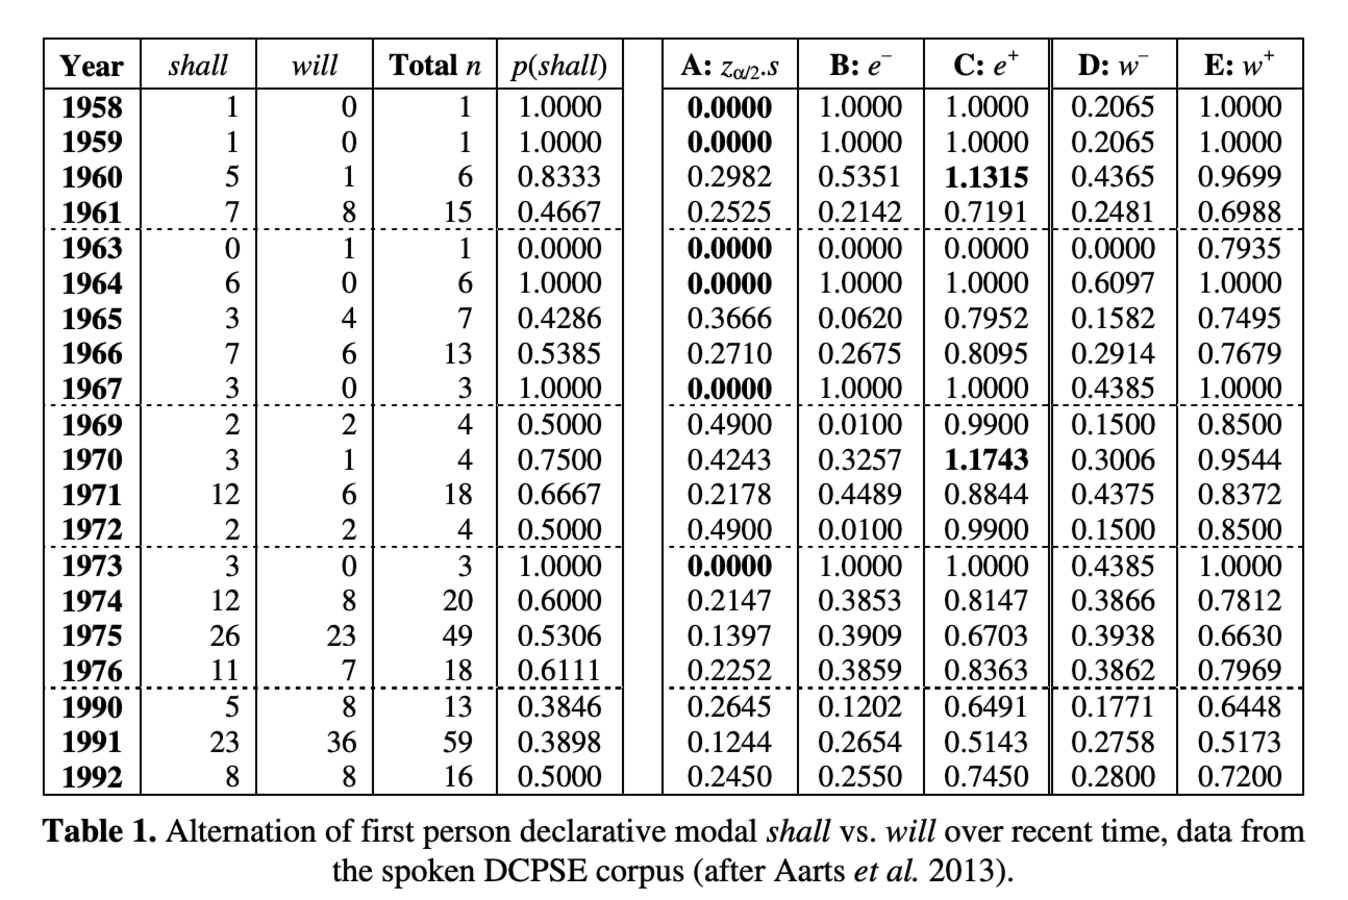
\includegraphics[scale=0.4]{wilson_chart.pdf}
    \caption{A paper about confidence intervals published a chart of values for
    the Wilson score interval~\citep{wallis2013binomial}, in the last two columns. Using $n$ and $p$
    for a $95\:\%$ confidence interval, we can quote this chart and compare with
    our code's output as a unit test.}
    \label{fig:wilson_chart}
\end{figure}

\begin{lstlisting}[language=R]
wilson_score_interval <- function(p, n, confidence) {
  z <- qnorm((1 + confidence) / 2)
  fixed <- p + z**2 / (2 * n)
  shift <- z * sqrt(
    (p * (1 - p) + z**2 / (4 * n)) / n
  )
  denominator <- 1 + z**2 / n
  list(lower = (fixed - shift) / denominator,
       upper = (fixed + shift) / denominator)
}

paper_numbers = data.frame(list(
  n = c(
    1, 1, 6, 15,
    1, 6, 7, 13, 3,
    4, 4, 18, 4,
    3, 20, 49, 18,
    13, 59, 16),
  p = c(  # "Total n" column
    1, 1, 0.8333, 0.4667,
    0, 1, 0.4286, 0.5385, 1,
    .5, .75, 0.6667, 0.5,
    1, 0.6, 0.5306, 0.6111,
    0.3846, 0.3898, 0.5),
  w_minus = c(  # "p(shall)" column
    0.2065, 0.2065, 0.4365, 0.2481,
    0, 0.6097, 0.1582, 0.2914, 0.4385,
    0.15, 0.3006, 0.4375, 0.15,
    0.4385, 0.3866, 0.3938, 0.3862,
    0.1771, 0.2758, 0.28),
  w_plus = c(  # "D:w-" column
    1, 1, 0.9699, 0.6988,
    0.7935, 1, 0.7495, 0.7679, 1,
    0.85, 0.9544, 0.8372, 0.85,
    1, 0.7812, 0.6630, 0.7969,
    0.6448, 0.5173, 0.72)
))


test_that("paper numbers match computed", {
  confidence <- 0.95
  result <- wilson_score_interval(
    paper_numbers$p, paper_numbers$n, confidence
  )
  tolerance <- 0.001
  for (i in 1:length(result)) {
    expect(abs(result$lower[i] - paper_numbers$w_minus[i]) < tolerance,
           paste("no match:", result$lower[i], paper_numbers$w_minus[i]))
  }
})
\end{lstlisting}

Argument by authority isn't wrong. It's just weaker than having
more thorough support for what we expect from a function.
In the example above, it also makes that claim only for a few,
select values, that are well away from edge cases.
Even so, it's good enough to make that claim that the
function-under-test was right at least once.


\subsubsection{Known at certain values}

Not every parallel implementation is a brute-force retelling
of a model. Most mathematical functions provide finger-holds
support of their correctness.

The simplest of these are parameters for which a function
takes a known value. The function could be a mess of
polynomials of trigonometric quantities,
\begin{equation}
  y = (\sin x)^3 - 6 (\cos x)^2 + 2,
\end{equation}
but these simplify considerably at $x=0, \pi/4, \pi/2, \pi,$
and so on. If the function should divide by zero for some
number, then that, too, is a parameter for which the function
has a known value, an exception.


\subsubsection{Inverse problems}

A lot of important scientific code looks at evidence and infers
what must have caused that evidence. This kind of inference is
called an inverse problem because it looks backwards from effect
to cause. Examples include regression of points to find a slope
and intercept, disaggregation of grouped data into finer groups,
and more classic inverse problems, such as calculating the density
of the earth from its gravitational field.

While inverse problems are mathematically difficult, they create
an opportunity for unit testing. I can simulate the
problem, from physical system to its evidence, and then ask
the inverse problem to return something close to the simulation
I created.

Let's make a survival analysis example. I have laboratory data
on the number of days between the birth of a new brood of mosquitoes
and the day on which each one dies. I've created a function that
takes two arguments, the number of deaths per day since birth,
and the temperature each day since birth. It returns a fit that
tells me parameters for a gamma distribution of probability of
death and a covariate effect for the temperature.

\begin{lstlisting}
def mosquito_survival_fit(deaths_per_day, daily_temperature)
\end{lstlisting}

\noindent{}The given function should give an exact fit if
the distribution of deaths is actually gamma-distributed and
if the dependence on temperature is actually linear. We can
construct that test by generating deaths using the hazard for
a gamma distribution and applying a linear effect with temperature.

When we make data to use in an inverse test, it's a little different
than actually simulating the data. I don't want to draw random
numbers the way I would for a simulation. I would prefer that
the values be evenly spread over all probable outcomes so that
there are no outliers. One way is to generate values from a
distribution using inversion. For instance, if a probability
distribution, $f(x)dx$ has a cumulative distribution function
$F(x) = \int_0^x f(s)ds$, then start by creating a set of $N$
values, $U=n / (N + 1)$ for $n=1\ldots N$. Then set $x$ by
solving $U_i = F(x_i)$.

For different problems, I'm looking for different ways to 
make the inverse problem nearly-exact. For instance, if I need
points distributed in space, a Sobol sequence gives pseudorandom
values that are mostly-even through space. If the inverse
problem is looking for a smooth fit to points, I try a forward
simulation that's purely linear or that has noise applied that
has values above and below the line by the same amount.
By creating a forward simulation that's well-behaved, I
create an inverse problem that can be close to the original.

The discussion, thus far, has treated every function as an
equivalent challenge. Computing the distance between points
on the earth with the Haversine formula is a challenge of much
different size than a meta-regression of cancer surveys.
A function that doesn't call other functions, besides maybe
some trigonometric library functions, is a low-level\index{low-level} function.
A function that calls functions that, themselves, call functions,
is a high-level\index{high-level} function. The \lstinline|main()| function is
the highest-level function.

Inverse problems are wonderful points to test because they
tend to be high-level functions. If tests pass here, that means
that, for at least this case, all of the functions below
have done their job well-enough that their faults aren't
visible to this test. I like to build trust in functions by
testing both parts and whole, but high-level testing addresses
a broad range of risks with fewer tests.



\subsection{Code it twice}

\subsubsection{Language and libraries}

It may seem like a chore to translate code from one language
to another, but it's an opportunity to find faults in the code,
if you're careful with the process.

We generally find faults in code by reading it during reviews, by testing
it, and by running it. Translating code to a new language requires
a very close read, so it serves as a review for off-by-one errors,
loop invariants, and the logic of branches. Something as simple
as changing counters from 1-based in \rlang to 0-based in \cpp
can bring your focus to every index in a method.

We also get to see how the code interacts with a new set of
libraries that support it. For instance, the generalized matrix pseudoinverse
function built into \rlang returns the Moore-Penrose pseudoinverse\index{pseudoinverse}
by default, while the one in Python~2.7 returned one of the three
other kinds of pseudoinverses. That took me
a full day to figure out, but the function-under-test is better
for that work.

Rewriting a function in a new language is most fruitful
if you adapt a core guideline from refactoring, which says that,
at each step, you should either move the code around or change
its functionality. By not doing both at the same time, you reduce
your mental load. For rewriting code, that means you rewrite
the same functions, with the same testable structure, before
you adapt those functions to idioms of the new language.

It's reasonable to keep code from a different language in
the unit testing suite, to execute it as part of those unit
tests, for direct comparison.


\subsubsection{Operating system platform}

I was tasked with porting high-performance computing applications
(like Charm, Lammps, VASP) from Linux to Windows, and the Intel
compiler's porting manual had an aside that porting an application
from one operating system to another improves the quality of a code base.
I hadn't thought about it before, but I had been seeing bug
after bug that came from undefined behavior in \textsc{c} code or
from a lack of specificity about library implementations (such
as arc tangent).

Running code on a different operating system creates problems
for parts of the application that do multi-threading, networking,
and file systems, all the parts that interact with the world outside
the application and are outside the scope of this document.

Changes that affect the science part of an application will
be floating-point types, as usual. They will be the common float exceptions
and how faults in mathematical code become failures for that code.

Some correctness problems in scientific code come from ways
the compiler can fail to deliver its promise to faithfully
add, subtract, multiply, divide, and round. This seems like
a promise the compiler would keep, but some compiler optimizations
can be risky because they assume the code they optimize will
be well-behaved. Ill-behaved code can be what \cpp calls
``undefined behavior,''\index{undefined behavior} such as dereferencing a null pointer
or failing to return a value from a function that declares
it does return a value. Most of the time, it comes from code
that has a mistake, but it's a mistake that one particular
compiler, or one particular set of compiler flags, avoids
turning into a failure.

Therefore, running code on different operating systems tests
the code's model of its runtime. That is how the code imagines
it will be supplied with memory and how it imagines threads
will work. It's how the code expects a divide-by-zero to return
an $\infty$ or $-\infty$ instead of raising an exception.
By running the code on different operating systems, we ask
whether it makes reasonable, conservative assumptions about
that model of the runtime, or whether it is prone to error.

We discover compiler and operating system problems when we
change hardware architectures, change operating systems,
change compilers, or change compiler flags. This can happen
twenty times a day if you run code on a cluster that has
a heterogeneous set of hardware architectures. Even CPUs with
the same brand, the same product name, and different stepping
numbers (fraternal twins, not identical twins), can react differently
to the same code.

As a result, we can also think of testing as reassurance that this
code runs well today, on this system. The \ieee standard 829--2008
calls this checkout\index{checkout testing} testing, 
``testing conducted in the environment to ensure that a
software product performs as required after installation.''
I haven't seen experience studies that show what tests will most
reliably expose failures during checkout. Because most of
the time, I'm running checkout tests on the same software
and operating system, but heterogeneous architectures, I expect
that problems will arise from differences in how they support
\textsc{mmx} routines, the set of machine language to support
multimedia instructions. These are crucial to speed for scientific
code and vary widely across versions of chips. I run checkout
tests on every new machine, so I want them to be just a subset
of the full test suite, so I choose tests that are
happy paths of the most mathematically-intensive functions,
and hope for the best.


\subsection{Traverse math choices}

\subsubsection{Form of equations}
Sometimes I decide it would be cooler to rewrite a polynomial,
\begin{lstlisting}
a0*x^3 + a1*x^2 + a2*x + a3
\end{lstlisting}
so that it's in Horner form,
\begin{lstlisting}
((a0*x + a1)*x + a2)*x + a3
\end{lstlisting}
as though the compiler couldn't figure that out on its own.

If I rewrite a function to use Horner form, and then I test
the former version against the new one, it tests parenthesis
placement.

More seriously, it can make sense to switch from one parameterization
to another, such as switching from the negative binomial for
$k$ failures
\begin{equation}
f(k;r,p) = \genfrac(){0pt}{2}{k+r-1}{k}p^r(1-p)^k
\end{equation}
to the negative binomial for $n$ trials,
\begin{equation}
f(k;r,p) = \genfrac(){0pt}{2}{n-1}{r-1}p^r(1-p)^{n-r}.
\end{equation}
You can get the same work done with both versions, but you have to
juggle the parameters differently, and each one is clearer for
different situations.

If I rewrite a function to use an alternate version of the
negative binomial, it tests the code to setup the parameters,
make the call, and interpret samples from that distribution.
It's a test of whether the code is typed correctly but also
a test of how the math is used. The differences in the two
distributions are about interpretation of a stochastic process.

There is a principle in statistics that if a variable must
be between zero and $k$, then uncertainty in that variable is bounded
by $k$. Similarly, we can't say here that either implementation
of a function is correct, but they do agree with each other.


\subsubsection{Stage of derivation}


Let's say we are supposed to calculate the mortality rate
for five-year age groups from birth to eighty years old,
for a Gompertz-Makeham mortality law. The parameters are
$(x, \alpha, \beta, \lambda),$ intermediate values are $(\mu, S)$ and the result is ${}_nm_x$.
\begin{eqnarray}
  \mu(x) & =&  \alpha e^{\beta x} + \lambda \\
  S(x) & = & \exp\left(-\lambda x - \frac{\alpha}{\beta}\left(e^{\beta x} - 1\right)\right) \\
  {}_nm_x & = & \frac{\mu(x+n) S(x+n) - \mu(x)S(x)}{S(x) - S(x+n)}
\end{eqnarray}
Wherever this equation comes from, whether it be a book or a
\textsc{png}\ in a Jira story, we can identify risks in transliterating
these equations to code. The most likely faults are improperly grouping
algebraic operations, mistaking signs, and forgetting terms. 

We can address those risks by returning to the first step of writing
a scientific function, which is how we represent the mathematical model.
The equations above are the result of integrating a function that has fewer
steps, even though it would be slower to run.
\begin{eqnarray}
  \mu(x) & =&  \alpha e^{\beta x} + \lambda \\
  {}_nm_x & = &\frac{\int_{x}^{x+n}\mu(s) \exp(-\int_{x}^s\mu(a)ds)ds}{\int_{x}^{x+n}\exp(-\int_{x}^s\mu(a)ds)ds}.
\end{eqnarray}
The resulting ${}_nm_x$ should be the same as that above within
machine precision, where machine precision means that we expect a drift
of about one machine epsilon for each step of the integration. That means
it should agree within several thousand times machine epsilon.

This new version could have its own faults and its
own corner cases, but they are unlikely to be the same faults
as the original function. This is a tremendous improvement over
not having such a test.

There are many possible parallel implementations. For this example,
we could make the looser assertion that the relative error of ${}_nm_x$
to $\mu(x)$ should be less than some cutoff. It's not as strong a test,
but it's quick to write.

What to test with brute force computation, and how to brute
force that computation, depends on risk assessment, time, and
whether your work is to question faults in the code or faults
in the model.


\subsubsection{Representation of physical system}

I mentioned earlier a birth-death model for voles. I could
write the math as an ordinary differential equation or I could
write the math as sampling a probability distribution for any single
vole to give birth or die. These are two very different representations
of the same biological system. The first is deterministic and applies
to large populations. The second is stochastic and applies to
populations of any size.

If we think of one of these representations as a test of our
implementation of the other, we need to use our criteria for
a good test. Ask what are the largest risks in an implementation
and how the second representation limits those risks by giving
us more precise expectations of its behavior.

Such a comparison would be a high-level test, so it would exercise
a lot of code. It would test algorithmic errors and decision errors
in all of that code. That's an efficient use of testing, but it also
has drawbacks. Small faults in some functions may cause minor
changes to a resulting value, too small to make a test fail
in one instance, but possibly a problem for a different set
of parameters. A high-level test can also make debugging different
if the test fails, because there is more code to search for
the problem.

The larger challenge is that two different representations of
the same model are sometimes supposed to disagree. Let's say
we ran the stochastic model of the voles a million times and
computed an average behavior. This will converge to the ordinary
differential equation at a known rate, as the number of draws
increases. However, there are some parameter regimes, such
as very high growth rates, coupled with very high death rates,
that can result in chaotic behavior, only in the stochastic system,
so that average values will no longer agree. It can be hard
to treat a unit test as a test of the code when the math
won't always line up.

If we make two fully-different implementations, we often don't
echo all of the options and flags from one to the other, so we
don't get good testing for all decision points. We may not
get an exact match at each value, either.

By the time we write a unit test that compares two representations
of a system, we have refined our understanding of the behavior
of the mathematical equations, in order to apply that expectation
to their implementation in code. When it works, it's a strong
affirmation. When it doesn't work, it calls into question how
much I understand about either mathematical model or numerical
analysis of the ensuing code. This is where a walk up the
implementation stack for scientific code walks into questions
about the science.


\subsection{Regression tests}
The simplest form of parallel implementation is to compare the output
of a function with the output of a previous version of the same
function. We can do this any time we make a change to a function.
It's a form of regression testing, a reassurance that the code
didn't get worse than it was.

Every form of parallel implementation mentioned above is a form
of regression testing.
There is a book called \emph{Release It!} that says we should
``make regression testing easy,''~\citep{nygard2018release}.
It's possible to make unit tests that file away a copy of
their output for comparison with future versions, and this is
very handy for refactoring steps.
The challenge is that, even if
they save output from functions, it takes work to figure out
\emph{how} a result changed if it did change. If the result
is a data frame, every value could have changed, or some subset.
Given which part of an output changed, the next step for the
developer is finding the fault.

Regression tests of high-level functions raise the question
of which, of all the low-level functions called, has a fault.
As a result, regression testing tends to be most effective
somewhere in the middle range of functions. That is, I test
functions that do enough work to be interesting but not so much
work that I can't imagine how all of the steps affect the output.
The output of high-level functions will change every time you
change the code, so they don't provide a good signal of problems.

The benefit, and threat to efficiency for testing, is that
parallel implementations of a function can lead to scientific
questions. Good unit testing strategies limit testing to the
highest risks in the software, and that principle applies
especially to use of parallel implementations, so let's
look at how alternative choices probe faults in code.



\section{Testing traits of a function}

\subsection{Measuring closeness}

If I want to test whether $a$ and $b$ are close to each other,
the absolute\index{absolute error} error between them is $|b-a|$, and I can write a unit
test by estimating how large a difference between them is reasonable,
given the number of calculations involved.
\begin{lstlisting}
function absolute_error(a, b)
    abs(b - a)
end

assert absolute_error(a, b) < 1e-7
\end{lstlisting}
Unit tests more often use relative\index{relative error} error, because it asks what
fraction the result is of the accepted answer, $|(b - a) / a|$.
\begin{lstlisting}
function relative_error(a, b)
    abs((b - a) / a)
end

assert relative_error(a, b) < 1e-3
\end{lstlisting}
This is particularly helpful because floating-point types carry
significant digits. That means they offer good relative error,
no matter whether the value is near $10^{-5}$ or $10^5$. We test
them using the machine epsilon and relative error.
\begin{lstlisting}
assert relative_error(a, b) < 1000 * machine_epsilon
\end{lstlisting}
Every language has a library function that will tell you the
value for machine epsilon, which is the smallest fraction that
one floating-point type can differ from another, as a relative
error.

If we need to compare one vector of values with another, then
we could require the error between each pair of values be less
than a given number. The easiest way to do that is by using
what's called an $L_1$ norm, meaning we calculate the absolute error and
look at its maximum. The same technique works for relative error.
\begin{lstlisting}
function l1_norm(x_vector, y_vector)
    max(abs.(x_vector - y_vector))
end

function l2_norm(x_vector, y_vector)
    max(abs.((x_vector - y_vector)^2))
end
\end{lstlisting}

A more interesting question is whether two vectors are a little
bit off from each other everywhere. To answer this question,
we sum the absolute or relative errors and put a bound on that
sum.
\begin{lstlisting}
function sum_of_squared_error(x_vector, y_vector)
    total_error = 0.0
    for i in 1:length(x_vector)
    	total_error += (y_vector[i] - x_vector[i])^2
    end
end
\end{lstlisting}


\subsection{Continuity}

Another kind of limit is the distance between function results
as the function inputs get closer to each other. We can often
find faults in a function by testing continuity of the output.
Here, a good unit test would mirror the definition of Lipshitz continuity.
\begin{lstlisting}[language=python]
C = 2.0
for (x1, x2) in [(0, 1), (0, .1), (0, .001)]:
    assert f(x2) - f(x1) < C * (x2 - x1)
\end{lstlisting}
The \lstinline!C! variable is a bounds on the slope for any
pair of numbers.

\subsection{Approach to limiting values}

Sometimes a limit of a function is the same limit you know
from high school precalculus,
\begin{equation}
  \lim_{x\rightarrow\infty} f(x).
\end{equation}
Maybe the limit goes to zero, or to 3, but the principle is
the same. You can test that a function is near the limit
as the value gets larger, or closer to zero. Better, you can
test that the function gets closer to the limit as the
parameter gets closer to its limit.
\begin{lstlisting}[language=python]
for (x1, x2) in [(pi, 100), (pi, 1000), (pi, 10000)]:
    assert abs(f(x2) - x1) < abs(f(x2 / 10) - x1)
\end{lstlisting}
This kind of convergence test can be more sensitive to
numerical accuracy problems than a simple test
that \lstinline|abs(f(10000) - pi) < 1e-5|.

We can know the limiting value of a
function, but we can also know how the function approaches
that limit. Another precalculus friend, the Taylor series
writes a function as a sum of terms that get smaller,
\begin{equation}
  f(x_0+x) \approx f(x_0) + \frac{f'(x_0)}{2}x + \frac{f''(x_0)}{6}x^2.
\end{equation}
If we know the first term in the series, then the second term
is a good guess for how far the function's output should be from
the limiting value, as a function of $x$.
\begin{equation}
  f(x_0+x)  - f(x_0) - \frac{f'(x_0)}{2}x \approx \frac{f''(x_0)}{6}x^2.
\end{equation}
We can create a test that takes a series of values,
$f(x_0+x)$, and takes the logarithm, in order to check that
the slope is $2\log(x)$ and has the expected intercept.
\begin{equation}
  \log\left(f(x_0+x)  - f(x_0) - \frac{f'(x_0)}{2}x\right) \approx \log\left(\frac{f''(x_0)}{6}\right) + 2\log x.
\end{equation}
The third-order term will create noise, but we've created a
test on the second derivative of how a function approaches a
value, which is a stringent test, even with noise.


\subsection{Using symmetry to test a function}\label{sec:symmetry-test}

Sometimes knowing the math of a software function lets you
test the software, even when you have an oracle problem.
\emph{Metamorphic testing}\index{metamorphic testing} uses the symmetry of the math function
in order to test the correctness of the software function~\citep{ding2016,guderlei2007,kanewala2015,liu2014}.

The mathematical description of a function is that it relates
a domain (input) to a range (output). We write $f(x) = y$.
If the function is an exponential, then $e^{-x} = 1 / e^x$,
so $f(-x) = 1 / f(x)$. We may not know what the value of
$e^{2.4}$ is, but we do know it has to match $1 / e^{-2.4}$.

Here's a longer example. Given a mortality rate, $m$, the
mean age of death over an age interval, $n$, is
\begin{equation}
    a = \frac{n - n(1+m n)e^{-m n}}{1 - e^{-m n}}.
\end{equation}
If we notice that this equation can be written
\begin{equation}
    a = f(m, n) = n  f_1(m  n),
\end{equation}
then we can design an interesting test.
\begin{eqnarray}
    \frac{a}{n} &= &f_1(m  n) \\
    \frac{a/2}{n/2} &= & f_1((2  m)  (n / 2)) \\
    a /2 &= & (n/2) f_1((2  m)  (n / 2)) \\
    a &= &2 * f(2m, n/2) \\
    f(m, n) & =& 2 * f(2m, n/2)
\end{eqnarray}
This result isn't true for almost all functions. It's a strong test
of the implementation. It's an example of the more general
form of symmetry testing, which insists that some transformation
of the inputs has a relationship with some transformation of the 
outputs,
\begin{equation}
    f(g(x)) = h(f(x)),
\end{equation}
where $f$ is the function under test, and $g$ and $h$ are the transformations.

\begin{lstlisting}[language=R]
mean_age_of_death <- function(m, n) {
  (n - n * (1 + m * n) * exp(-m * n)) / (1 - exp(-m * n))
}
test_that("dividing by a constant multiplies by a constant", {
  m1 <- 0.01
  n1 <- 1.0
  a1 <- mean_age_of_death(m1, n1)
  for (k in seq(0.1, 5, 0.3)) {
    a2 <- mean_age_of_death(k * m1, n1 / k)
    expect_lt(abs(2 * a2 - a1), 1e-7)
  }
})
\end{lstlisting}

The metamorphic\index{metamorphic testing} relation between $m$ and $n$ ties these two together
for parameter testing, too. It means that $(m=2, n=0.5)$ is in the same
equivalence\index{equivalence class} class as $(m=0.5, n=2).$ Knowing
metamorphic relations reduces the space of parameters to test.

One way to use metamorphic relations is to rewrite a function, when possible,
so that there is an outer function that takes parameters in a form that's
convenient for the caller and an inner function that takes the reduced
set of internal parameters. This means we create a
\lstinline|mean_age_of_death(mn)|, and test that separately.

Metamorphic testing is an assertion about a symmetry relationship between
the domain and range of a function. Because it's an invariant at the top-level
of the function, it has an opportunity to find simple faults in algebra,
grouping of terms, or off-by-one errors. It also has an opportunity to
find faults that result from denormalization or loss of significant digits
in floating-point math.


\subsection{Units as symmetry}

Almost every program has symmetry relationships that can be used
to either improve testing or, alternatively, simplify the program in
order to reduce risk. We specify programs with lots of parameters,
but the underlying equations depend on combinations of those
parameters. Physicists find insight in how parameters combine
to \emph{scale}\index{scaling} an equation~\citep{barenblatt1996}.
The techniques for finding how parameters combine are called
nondimensionalization\index{nondimensionalization}. It's a
well-understood set of steps to use for any math equation, especially
for differential equations.

The central idea of nondimensionalization is that every physical
law (or biological law, epidemiological law, whatever) can be
written as a function of dimensionless independent variables
and a set of parameters, and it returns dimensionless variables,
which are, themselves, scaled by parameters to produce the result.

Let's take the mean age of death, above, as an example.
The physical law is the function we called $f_1$.
Recall $a/n = f_1(mn)$.
The dependent variable is a time, so it has time units, $[T]$.
The independent variable, the mortality rate, is a rate,
so its units are inverse time, $[T^{-1}]$.
The duration of an age interval is the only parameter, a time, $[T]$.
Every argument to $f_1$ has no units and it returns a result with no units.

In practice, you can nondimensionalize an equation by replacing
each variable, $x$ by $x=\bar{x}/k_x$, where $\bar{x}$ is the
nondimensional variable and $k_x$ is the scaling constant. Sometimes
it's helpful to add an offset, $x=(\bar{x} - x_0)/k_x$. Then
push the constants around the equation until they sit near each
other and choose values for the arbitrary new constants, such as $k_x$,
that set groups of constants to the value one.

If you're familiar with how vector subspaces work, then
you can work out some of the details for yourself.
Picture a vector subspace with dimensionality equal to the
number of base units of the parameters, so we include
length, $[L]$, time $[T]$, mass $[M]$, and so on, if they are used
by the given parameters. Each parameter's units can be described
by a vector in that space, acceleration would be a $[LT^{-2}]$, or
a vector $(1, -2, 0)^t$. If we make a matrix using a column
for each parameter, then the number of nondimensional parameters
is the size of the nullspace of that matrix. For $n$ parameters
and $m$ base units, there will be $n-m$ nondimensional parameters.

There is some history to using nondimensional parameters in
computations. Early computers didn't have a floating-point type.
They used fixed-point\index{fixed-point type} types, which are represented as integers
with a known scaling value. You can think of them as floating-point
values that all have the same exponent. If you want to compute
with types like this, it helps to know that all of the values
are somewhere near one. They can be ten times as large or ten
times as small, but you try to scale the inputs so that
computations are near one and then rescale the outputs at
the end before returning results.

Somewhere between the use of fixed-point types and discovery
of how beneficial it is to reduce parameters by scaling
equations, a motto was born, ``Computer code is always
dimensionless.'' By organizing code so that the inputs are
rescaled, at the start, into dimensionless parameters and
rescaled independent values, the risk associated with
mistaken units is all placed into one, testable area.
The rescaled, dimensionless central computation then has
fewer parameters to test. The process pushes our understanding
of the problem into code with clearer, testable expected
behavior.


\section{Statistics for testing}\label{sec:statistical}

\subsection{Stochastic functions}

% Scope. The problem in front of us.
Some functions should produce random outputs. Take, for instance,
this model of an aquatic life stage for insects. We assume that
a small initial insect population will tend to increase until
it reaches a carrying capacity. If the population is above carrying
capacity, individuals will die at a higher rate until it is lowered.
For this example, we theorize that the carrying capacity changes
randomly and the population responds to those changes. This
means the population will rise and then bounce around
some average value, as shown in Fig.~\ref{fig:insectrise}.

\begin{figure}
\centering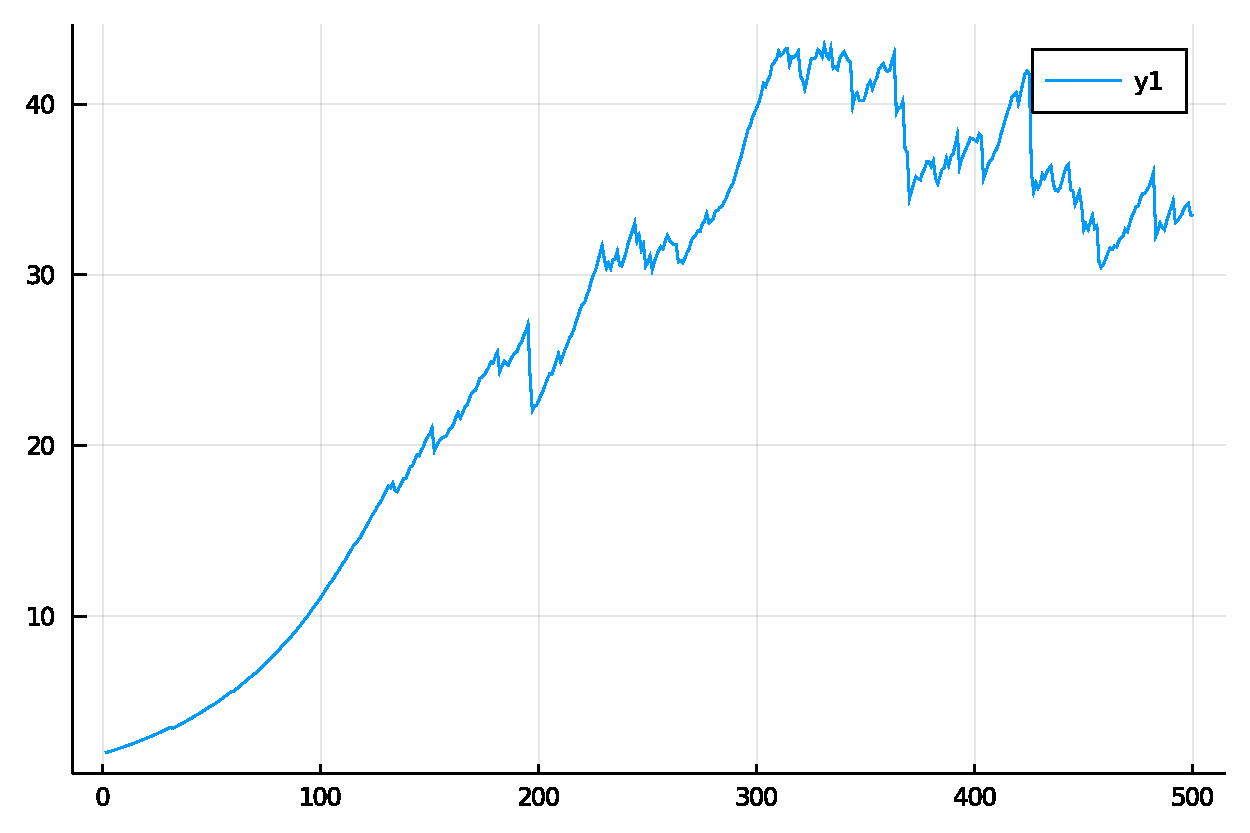
\includegraphics[width=4in]{insects_rise.pdf}
\caption{This is a stochastic model of the growth of a
population, where the population's carrying capacity changes
randomly with each time step. It rises in fits and starts.\label{fig:insectrise}}
\end{figure}

\begin{lstlisting}
beverton_holt(x, K, nu) = (nu * K * x) / (K + (nu - 1) * x)

function beverton_holt_stochastic(young, carrying, params, step_cnt, rng)
    carrying = zeros(Float64, step_cnt)
    alpha, beta = [params[:food_alpha], params[:food_beta]]
    rand!(rng, Distributions.Beta(alpha, beta), carrying)
    carrying .*= params[:max_carrying]

    x = zeros(Float64, step_cnt)
    x[1] = young
    for step_idx = 1:(step_cnt - 1)
        x[step_idx + 1] = beverton_holt(
            x[step_idx], carrying[step_idx], params[:growth_rate]
            )
    end
    x
end
\end{lstlisting}

A function like this is its own miniature experiment. If the
carrying capacity were constant, the result would be a
discrete-time approximation to a logistic function. Given the
random carrying capacity, I don't know what values it should
produce, but they should be both above and below the carrying
capacity, not quite centered on it because growth is exponential.

There are two problems, then, for testing this function.
One is that every time I run the function, it will return a different
set of results. The other is that, as we have seen for deterministic
scientific code, I don't know exactly what the mean of the
distribution of values should be. I have only expectations about how
this function should relate to other functions.

We're going to reach for some statistical tools to help
to characterize the output of random functions. The main
contribution here is to clarify how software tests are used
at different stages of software development. Clear goals
make for better use of statistical tests. Before covering
those stages, we use the nymphs to remind ourselves of the
basic statistics.

\subsection{Statistics primer}

When a function has a random output, that function has
a true distribution, and the output is a sample of it.
We use the output to infer the probability that the true
distribution has some property.

For instance, the aquatic life stages, above, give us a
time series. We could look at the behavior of those stages
over long times, as shown in Fig.~\ref{fig:insectlong}.
The population size bounces around some average value,
forgetting its initial starting size.
If we exclude the first thousand time steps, we can look
at the distribution of population sizes, binned as a histogram
in Fig.~\ref{fig:insecthist}. This is the distribution of
population sizes from a single call to the function.

\begin{figure}
\centering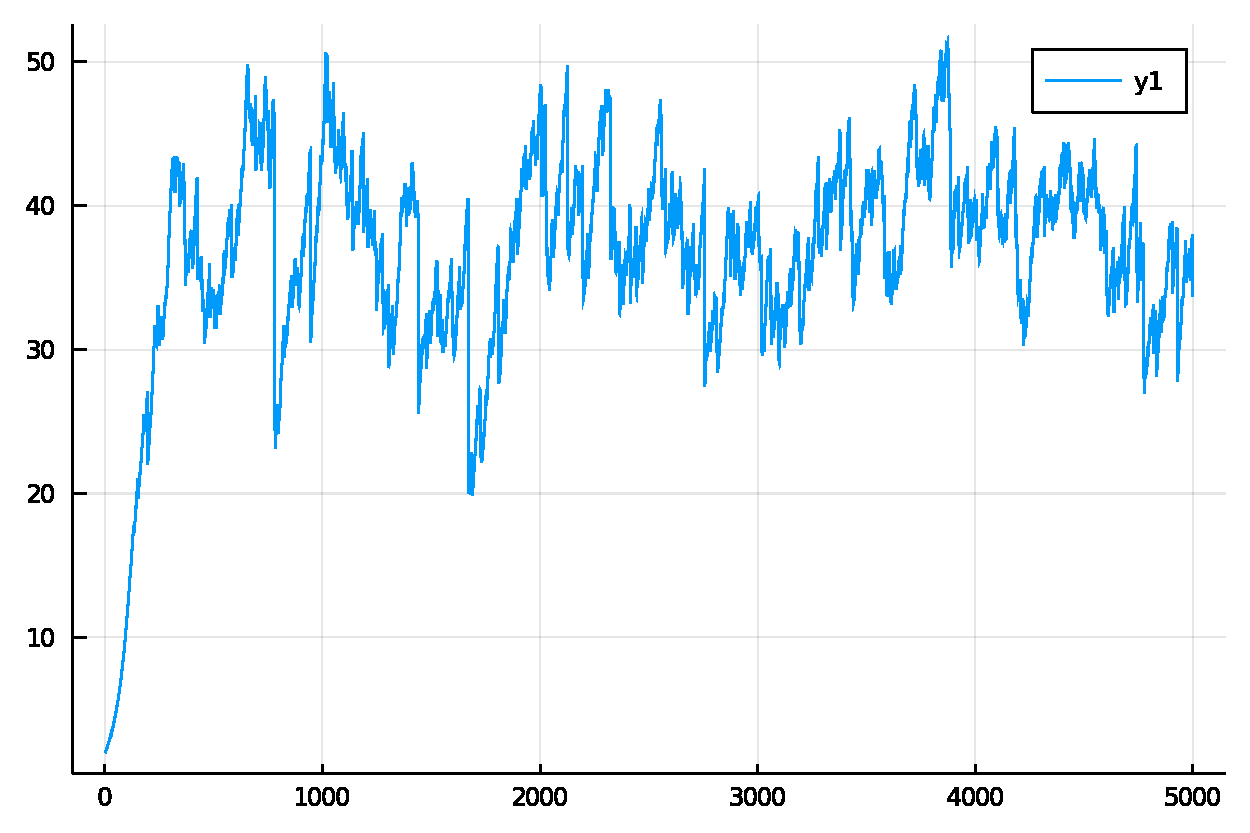
\includegraphics[width=4in]{insects_long.pdf}
\caption{Over longer times, the early rise in the population
is less important. The population varies around some average value.\label{fig:insectlong}}
\end{figure}
\begin{figure}
\centering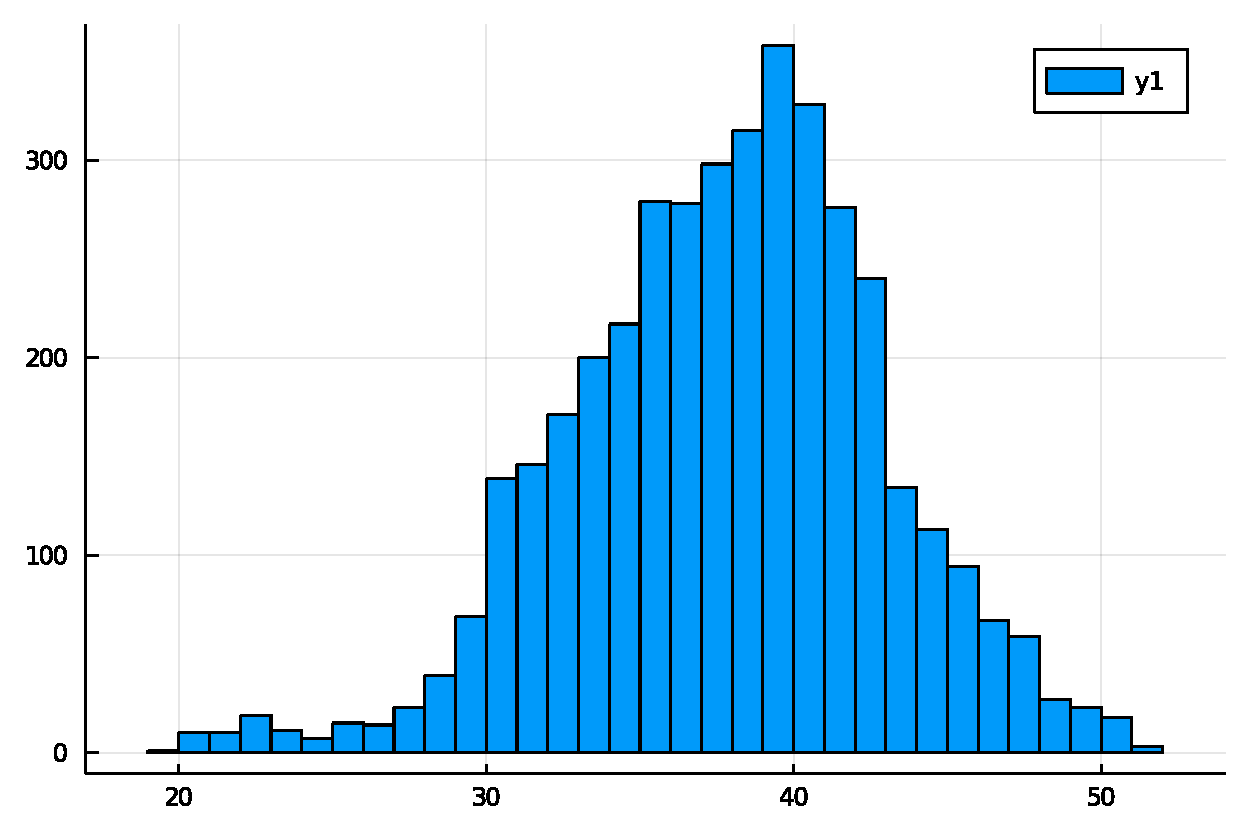
\includegraphics[width=4in]{insects_histogram_4k.pdf}
\caption{If we focus on long-time behavior and ask how often
the population is any given size, this function, for these
parameters, produces a particular distribution of sizes.\label{fig:insecthist}}
\end{figure}

The code in the function will tend to produce population sizes
that have some distribution. Each time we run it, the sample
population sizes will approximate the function's underlying
distribution. If we introduce a fault in the function, or if
it already had a fault, then the underlying distribution will shift,
but it may not be apparent from the samples that the underlying distribution
has shifted.

We approach this problem by reducing the problem to a simpler one.
Instead of asking whether the whole distribution of answers is different,
we measure one property of the distribution, and ask whether it is different.
Each of these properties is a single number, called a statistic.
There are three kinds of statistics that are standard: measures of
location, measures of spread, and measures of association.

\subsubsection{Measures of location}
The most common measures of location are the mean and median of the distribution.
The mean is the average value. For the function, there is one true
mean. Each time we generate samples, we estimate the mean using
\begin{equation}
  \mbox{mean}(\hat{Y}) = \frac{1}{N}\sum_i{\hat{Y}_i}
\end{equation}
The hat that turns $Y$ into $\hat{Y}$ indicates that we are looking at samples.
In \rlang, it's as simple as \lstinline!mean(y)! for an array of values.

If we sort the $\hat{Y}_i$, then we can identify quantiles, where the
5\,\% quantile is the value 5\,\% down the sorted list. There is some
ambiguity here, depending on whether the list divides evenly into the
quantile, and statisticians, in their passion for correctness, have identified
seven different ways to count a quantile. All of them are available
in the the \rlang \lstinline!quantile(y, percents)! function.
The most important quantile, though, is the median, which is 50\,\%
down the sorted list. Sometimes this can be more stable when the
stochastic function occasionally gives very large or small values.
The median and the mean are, in general different values.

Show measures of location on the example.

Each run of the stochastic function will return different samples
with a different mean. The more samples there are, the closer
the mean will tend to be to the mean of the underlying function.
There is a rule that says that if you want the mean of the samples
to be ten times more accurate, then you need to draw a hundred times
more samples.

\subsubsection{Variance, standard deviation}
When there is just one vector of random numbers coming out
of a function, it can be helpful to characterize how far
they are from their average value. The variance is
the average of how far each value is from the average of all
values,
\begin{equation}
  \mbox{var}(\hat{Y}) = \frac{1}{N}\sum_i (\hat{Y}_i - \bar{Y})^2,
\end{equation}
but you'd use the always-avaiable
as \lstinline!var! or \lstinline!variance! in any language.
The standard deviation is the square root of variance.

If variance is zero, then every value in the vector is
the same. There are some functions, such as the Cauchy
distribution, that don't have a variance. For such a function,
the value of the variance will keep increasing as the
number of draws of the function increases, instead of
converging to a single value. This, in itself, is a
testable property of a function.

\subsubsection{Measures of association}

Let's say the output of a function is a set of $y$ values,
and the input is a set of $x$ values. You may not know
how $y$ depends on $x$ exactly, but you know that it
does. The Pearson coefficient is a function of
$N$ $y$ values and $N$ $x$ values that will return a number
between -1 and 1, where -1 is a line with a downward slope,
1 is a line with an upward slope, and 0 means the points
are evenly arranged so that they don't slope up or down
and aren't collinear.

For a single $y$ that depends on a single $x$, the equation
is a few lines of code.
\begin{equation}
r_{xy} = \frac{\sum_i (x_i - \bar{x})(y_i - \bar{y})}{\sqrt{\sum_i (x_i - \bar{x})^2}\sqrt{\sum_i(y_i - \bar{y})^2}}
\end{equation}
It conveniently generalizes to more dimensions.

The Pearson coefficient is a handy, if imprecise,
set of guard rails on the behavior of a function.
It quickly determines whether the output rises or falls with the input,
even in the presence of noise. It can say whether the output
isn't linear enough, or whether it's too linear.
It even has a multidimensional generalization for data that
has multiple $x$ and $y$ values.

Apply Pearson to early behavior of the example.

Kolmogorov distance. Empirical distribution function?


\subsubsection{Confidence interval}

Assume there is a function with randomness, that produces floating-point numbers. Those results
have some average value, but they vary around that average value.
If we run this function a thousand times and take the
lower value, below which 2.5\,\% of the results fall,
and the upper value, above which 2.5\,\% of the results fall,
then this interval is the 95\,\% standard deviation.

For research statistics, the standard deviation is often part
of an argument that a model of a problem is appropriate to
the observed data. For unit testing the standard deviation
is a rule of thumb for how often a perfectly good unit test
will randomly fail. If you want it to fail five percent of
the time, use a 95\,\% interval. If you want it to fail
one time in a thousand, use a 99.9\,\% interval.

Given that results from a function are random, and we
want to make some cutoff on which results are acceptable,
we want to choose a cutoff that is informative, so it's
close to the average good value. On the other hand, we don't
want it to fail a lot. The standard deviation tells us
how much push luck in either direction.


\subsection{Initial development}

I don't know a name for the testing we do during initial development
of software. Whether I work in an electronic notebook, or an integrated
development environment, or on the command-line, I develop code using
a combination of functions and free code, with lots of plots to answer
lots of questions. There is certainly testing that happens at this stage,
and it's kind of an acceptance test, but it isn't run by a client or
stakeholder besides the author. It's the only testing some code will ever have.

There are two challenges during this stage of software development,
and they complicate each other. The first is that the goal of this testing
is to answer the question of whether the distribution of the underlying
function matches some known model. This could be a classic hypothesis test,
where the null hypothesis would be that the mean of a distribution has a
particular value, and we sample the function in order to gather evidence
to support the hypothesis that, for instance, the mean is higher (a one-sided test) or
differs (a two-sided test).

The good news is that, at this stage, the developer is committed to
ensuring this first writing of the code is correct. If it takes a day
to collect a million samples, then that could be reasonable. More samples
gives the test more power. The variance of the mean will become small,
and maybe that can reduce the risk that the function is incorrect.

The bad news is the second challenge. Like any other scientific code,
the code in a stochastic function doesn't necessarily have a particular
known true value for a statistic. That means we have to resort to the
other methods for testing scientific software, such as comparing
different versions of a function or looking at traits of a the function.
Does the answer go down when a particular parameter goes up? When a parameter
reaches a particular, limiting value, does the distribution take a known
shape? We not only have to write tests that capture our expectations
about a function, we have to do it in circumstances that say that, sometimes,
the test will give the wrong answer.

Given the context of initial development of a function, it's reasonable
to compute the coverage of a test. Run a 95\,\% coverage hypothesis test a hundred times
and ask whether about five of them fail. Time and attention are
an advantage here.


\subsection{Unit test}
When I convert that functional test into a unit test, I can encounter
a statistical challenge from the need for the unit test to be faster.
If I plan to execute a similar unit test for an array of input parameters,
then the function has to run many times per input parameter. I want that
number to be small enough to run quickly but large enough to be precise.

If you test by a cut, the size of the cut determines type-i and type-ii error.
Statistical hypothesis tests tell you the likelihood of those errors.
Coverage is the fraction of times that it succeeds, given type-i error.

We avoid this question, somewhat, by pinning random seeds and being
willing to re-investigate when the tests fail.
Set alpha large. Find a test that passes. Then bring the cut in,
so that power is high.

I make tests with random inputs, so they explore more alternative
paths in the code than I might guess. I run tests of random
functions a thousand times so that they have more chances to
show a real bug. Randomness in testing is a free source for
finding faults, and it's a constant headache.

In order to use the statistical tests above, I need to choose
a cutoff on what is a passing test and what is a failing test.
If I choose a cutoff that's useful for finding faults, it will
always fail for some percentage of tests. For a 95\,\% confidence
interval, it will fail 5\,\% of the time. Even for a
99.9\,\% confidence interval, it will fail once in a thousand
tries. This means the green lights of a unit test display will
be red without reason once in a thousand times, but that's
enough not to pay attention to a red light. It's a lure to
rerun the test suite every time there is any red light.
It's a waste of attention.

The solution is simple. Fix the seed for the random number
generator for each test that has randomness. The random
seed determines the exact set of random values that will
follow. If the test passes for a particular random seed,
then it will always pass for reruns of the unit test until
some fault is introduced.

The simple solution is sometimes impossible and always
disappointing. Most programming languages offer the tremendous
convenience of calling \lstinline!rand()! anywhere in the
code, which uses a global random number generator. Sometimes
\rlang code calls \lstinline!rand()! and then calls \cpp code
that calls \lstinline!rand()! from a different random number
generator. Authors
of code unfortunately use this convenience, creating side-effects
for testing. Only sometimes can we make a repeatable
stream of random numbers by declaring a specific random number generator
and passing it to a function.

(It's also possible to greatly reduce the rate of failure
for a statistical test, even with the same 99\,\% cutoff
on acceptable results, if we take the same hundred tests
and use the statistical framework to treat them as ten sets
of ten tests.)

Let's say we can fix the seed for a function, and for all the
functions it calls. The joy of randomized testing is that more
runs might yield more faults in the code. We
can still do lots of runs by creating a unit test that is run once
for a set of seeds.  The procedure is to define a starting seed and run against
the next thousand seeds. When the test shows no real faults,
choose a starting seed for which the next thousand all pass
the test within some tolerance. This is less simple, but it
explores the space of tests and is likely to signal when
a real fault arrives.


\subsection{Regression testing}

We use regression testing to ask whether a function's output has changed.
There is a former version of a function producing samples $A$ and a current
version of a function producing samples $B$. We construct a statistical
test to ask, for instance, whether the mean of $B$ differs from the mean of $A$.

As before, there are poor man's versions of these. For instance, we could
measure a statistic of $A$ very well and ask only whether $B$ agrees.
We could look at the values and decide, off the cuff, whether they are close
enough.

I'd like to emphasize here that, when doing comparison of two sets of samples,
we have an advantage over other goals. We don't have to use the mean and
variance. We can use more robust measures.

The trimmed mean is a statistic that sorts the samples, throws out
the top few and bottom few, and then takes the mean. For long-tailed
distributions, this can be much less susceptible to outliers. In \rlang,
this is built in as \lstinline!mean(y, trim = 0.2)! for a 20\,\% trimmed mean.

Hubert's M-estimator is similarly robust to outliers. For some distributions
it can be more stable than the trimmed mean. In \rlang, this is \lstinline!???!.

In both cases, if the function is slow to run, so that the unit tests
have time to collect few samples, it can be helpful to use a bootstrap
to estimate a statistic. Bootstrap techniques deal better with distributions
that aren't Gaussian. In \rlang, a percentile boostrap-t to estimate
a trimmed mean would be \lstinline!boot(mean)!.

If that kind of testing doesn't seem well-behaved, it's reasonable
to try ranked comparison.

All of these robust methods can be applied to unit tests, as well.
They require more computation from the statistics functions but
get more value out of each call to the function-under-test.

Lastly, regression testing of stochastic functions can benefit from
techniques called variance reduction. These are methods that artificially
reduce the variance of $\hat{B}_i-\hat{A}_i$ while giving a correct
result for measures of association for $\hat{B}_i-\hat{A}_i$. A simple example
is to make a copy of the random number generator. Then pass the same
random number generator into both versions of the function. If those
functions are sufficiently similar, if they make the same calls to the
generator in the same order, then using copies of the generator will
make their results more similar.

For one version of regression testing, you could ask whether the results
are exactly the same, given the same random seeds. That would
be reassuring.


\subsection{Acceptance testing and checkout testing}

I'll mention two more kinds of testing, checkout tests and acceptance tests.

A checkout test is a quick test that runs before doing computation on a new
computer, or after each compilation. It's especially useful when working on
a heterogeneous cluster, where different computers have different \cpu{}s or
different compiler flags. I'm doing a quick look for problems caused by
compiling for one architecture and running on a slightly different architecture.
There is a constraint on these tests to run quickly, but the question is
whether the answers are correct.

An acceptance test asks the same question we asked at the start of
the software process. Does this software give the correct results when
I give it a good, hard look? These tests often take a while to run and,
in the case of stochastic functions, will gather enough samples to have
good power.

In both cases, I can't expect that the test will yield the same answers
every time I run it. A change in compilers can change rounding modes
for floating point. A change in how code is linked can change the
random number generator. I can't rely on pinned seeds. There will
be a chance that tests fail with a type-i or type-ii error. I can minimize
those chances by using appropriate hypothesis tests. I can't make the
randomness go away.


\subsection{Conclusion}

As with all testing, testing of random functions is about finding the
appropriate strategies to reduce risk. Our chief method for simplifying
these tests is to be clear about the testing goal at each stage of
software development. During early development, sample so much that
the variance is small. During unit tests, find random seeds that are
within confidence intervals and pin them. During regression testing,
choose robust estimators with variance reduction.

There is no way to avoid proper statistics, however. As with other
challenges for testing scientific software, I test well when I know
the function-under-test well enough to quantify my expectations
about its behavior.



\section{Testing data movement}\label{sec:data-movement}

\subsection{Data movement}\label{sec:movement-movement}

We said in Sec.~\ref{sec:parallel-twice} that there are four
steps to writing a scientific function, representing the mathematical model,
preparing a discrete version, translating it to algorithms,
and writing the code.
Rarely is scientific software just one mathematical model
and just one ensuing algorithm. It's a series of models supported
by a series of algorithms.

For this software, as for any software, using the right algorithm
ensures speed and scalability, and the right algorithm depends on
its associated data structure. The relevant undergraduate class
is called Data Structures and Algorithms, always the two together.
As a result, performant scientific code is a series of algorithms
joined by a series of translations from one data structure to
another, each to support the next algorithm. The high-performance
computing crowd calls any such code \emph{data movement,} as though
it were replacing sets in the entracte,
but software engineers call it integration code and know that
integration testing is one of the most important kinds of unit test.


\subsection{Integration testing data movement}

A classic example of data movement is reorganizing a multidimensional
array from one axis ordering to another. An algorithm with nested
for-loops usually acts on nested axes. The order of the axes should
put those for the inner loops last (for \textsc{c} and Python which are row-first), or put those
same axes first (for \rlang and Julia which are column-first). This so
often controls the speed of an algorithm that it isn't considered an 
optimization to fix it but an error to fail to set the order.

More complicated an example would be translating a graph from
an edge-list representation to an adjacency matrix representation.
Both have their place, but the correct form depends on the
algorithm that will act on this data.

Data movement tends to stress performance of memory access
and integer arithmetic. It carries risks of off-by-one errors,
loop endpoint errors, and assignment errors. These are different
from the performance characteristics and likely faults in core
algorithmic code, so they suggest data movement should be in its
own function and should be tested separately, for both performance
and efficient testing.

This produces a mental model for a scientific application. It begins
with translating configuration parameters from their specification
to the values internally. Inputs are verified. Then the application
is a series of data movement, followed by algorithm, and data movement
for the next algorithm. Then results are written.

\subsection{The CRUD case}\label{sec:crud}

The prosaic brother to data movement is the ubiquitous selection
and editing of data frames when reading and writing data.
The data frame is the algorithmic equivalent of a minivan, more
about convenient pickup and drop-off than about getting from $A$
to $B$. When we edit data frames, during save or load, or during
data movement, the correct result is more a matter of software specification
than a matter of difficult calculation.

A good testing method for data frame manipulation, is therefore
unit tests that assert the output data frame meets a list of requirements.
There is, happily, a framework
for recording and conveying this work, the create-read-update-delete
(CRUD) list. For example, if we were editing a mortality data frame:
\begin{itemize}
\item \textbf{Create} - If the input data doesn't have excess mortality,
  then derive it from cause-specific mortality and prevalence.
\item \textbf{Read} - If the user specifies \lstinline!get_csmr!, then get cause-specific
  mortality from the database and add it to the data.
\item \textbf{Update} - Use the average of incidence data at all child
  locations because it tends to be sparse.
\item \textbf{Delete} - All-cause mortality isn't included in this step.
\end{itemize}
These are requirements. Failure to meet one of these requirements
often won't make the code stop running. It's no less wrong.

These tests are classic boundary-value tests, where
we try parameters at the lower boundary, upper boundary,
and middle of the range. Combinatorial testing can be appropriate
across all parameters, and we can often create a single data frame
where each row represents a different test.

\subsection{Example}
This example, in Python, is a function with two arguments, but both
are dataframes, just read from input files. Think of them as two spreadsheets
with multiple rows and column headers \lstinline!x_local!, \lstinline!a_data_id!,
and so on.
\begin{lstlisting}[language=Python]
def shift_priors(self, data, adj_data):
    """For subnationals, shift priors given parent run.

    Args:
          data (pd.DataFrame): All of the input data, including priors.
          adj_data (pd.DataFrame): Parent predicted data values.

    Returns:
        Data with adjusted priors.
    """
    integrands = data.integrand.unique()
    priors_from_draws = data[data.x_local == 0]
    unadjusted_data = data[data.x_local == 1]
    parent_predict = adj_data[
        (adj_data.x_local == 1) &
        (adj_data.a_data_id != IHME_COD_DB) &
        (adj_data.location_id == int(float(self.loc)))]
    shifted_priors = pd.DataFrame()
    for ig in integrands:
        ig_prior = priors_from_draws[priors_from_draws.integrand == ig]
        ig_data = parent_predict[parent_predict.integrand == ig]
        if len(ig_prior) == 0:
            pass  # No priors to adjust
        elif len(ig_data) == 0:
            # No fit with which to adjust, so keep the priors.
            shifted_priors = shifted_priors.append(ig_prior)
        else:
            ig_prior -= ig_data.mean()
            shifted_priors = shifted_priors.append(ig_prior)

    shifted_priors['meas_value'] = shifted_priors.meas_value.clip(lower=0)
    newdata = unadjusted_data.append(shifted_priors)
    return newdata
\end{lstlisting}

If we wanted to make a decision table for this function, what are
the possible values of each entry in each row of the input data?

\begin{center}
\begin{tabular}{|l|l|}
\hline Variable & Values \\ \hline
\lstinline!data.x_local! & 0, 1, not 0 or 1 \\
\lstinline!data.integrand! & same as another row, same as adjusted row \\
\lstinline!adj_data.x_local! & 0, 1, not 0 or 1 \\
\lstinline!adj_data.a_data_id! & \lstinline!IHME_COD_DB! or not \\
\lstinline!adj_data.location_id! & \lstinline!self.loc! or not \\
\lstinline!adj_data.integrand! & same as another row, same as data row \\ \hline
\end{tabular}
\end{center}

\noindent{}That makes $3\times 4 \times 3\times 2\times 2\times 4=576$ different inputs.
This excludes the effects of calling the function
\lstinline!adjust_prior_by_mean_of_fit()!.

What is the algorithmic complexity of this function? There is one
if--then--else, so the answer could be three, but each condition in a dataframe
selection is another path through the code. For instance,
\lstinline!data.x_local == 0! is a conditional with two outcomes, leading
to very high algorithmic complexity, hidden in data frame arguments.

A project manager can ensure good communication between the scientist and
developer by writing \textsc{crud} assertions in English.
\begin{itemize}
    \item[R1.] Read parent location's estimate of priors as ``adjusted data.''
    \item[U1.] Update adjusted data so that the mean of the priors for this location matches
        the mean of the data for this location. Keep the shape of the priors.
    \item[U2.] Update priors, after adjustment, so that they are greater
        than zero for all integrands.
    \item[D1.] Delete local adjusted data that doesn't match the current location.
    \item[D2.] Delete local adjusted data that doesn't match the integrands.
    \item[D3.] Delete local data for this location if there are no parent
        priors for the same integrand.
\end{itemize}
Then we can write tests that verify these \textsc{crud} requirements for
each of the 576 kinds of inputs.





\section{Outside the code}\label{sec:outside-code}

\subsection{Testability}

The six parts. Simple, observable, controllable, knowable. Line-by-line help (int, not unsigned, etc.) Voas and Miller. Vishal Chowdhary.

The most important non-functional qualities in research code are that it
is transparent and changeable. We want to be nimble and expressive
with our coding experiments. By the time this research code
becomes more established, we think more about ensuring efficiency
and that the code be usable. It should support optional ways to
call it. Somewhere in-between the birth of a new function and its
adoption into our library of code, we find ways to ensure its
correctness.

These conflicting priorities create tension in priorities.
More testing makes code more brittle. Early work is about
experimentation, and later work is about confirmation and
expansion of capability.


\subsection{Documentation defines what a function wants to be}

Sec.~\ref{sec:parameter-wilson}, on parameter testing, uses a function that's a hybrid
between Wilson's score interval and a Poisson estimator. That hybrid
doesn't have a name, and there's no paper or Wikipedia entry for it.
We can test that its output is a continuous function of its input
parameters. We can test that it matches known values for limiting cases,
but the right version of this function is the one that a team agrees
is right.

That team is usually not just the people in the room. It includes stakeholders
outside the room. It includes reviewers. It includes future versions of the team.

The tests can be a clear statement of the contract this function upholds.
So, too, can project documents, as mentioned in the data movement section,
where \textsc{crud} defines selection from a dataframe. 
Function documentation, in particular, is where the software
developer, the one who wrote the function, states their understanding
of the contract that function fulfills. It's the closest statement,
in English, of what unit tests should assert.

Like all other work, documentation takes time and is prioritized by
how it addresses risk. Give the highest-level explanation first.
This could be a reference to a paper, a book section, documentation from another library.
Then say \emph{why} this function exists and \emph{why} it works the
way it does.

And on the technological side, equations in documentation communicate
clearly with research-oriented readers. Similarly, code examples, run
as unit tests themselves, within the documentation, ensure always-working
examples for development.


\subsection{Team is critical to tests}

Take a function under test and project it onto a
screen at the front of a meeting room. Place around that screen
the team you have or the team you would like to have.
Engineering studies show that the future utility, or burden,
of that function depends no more on its testing than it
depends on the culture of that team~\citep{neumann2016,kanewala2014}.

Culture is beyond the scope of this document, but conversations
aren't. One point to raise in that meeting room could
be the effect of discretization or floating point representation
on the mathematical representation. Another could be a
description of statistical properties of the function, a set
of equations, beyond those to implement the function, that
describe its expected behavior. Someone could raise an observation
that brute force solution is suprisingly possible.
The team could discuss likely sets of parameters that might
matter, some determined by the math, some by logic in the
code. A product manager could supply \textsc{crud} requirements.
A systems engineer could describe the expected architectures
and risk of failure due to optimization levels. Every section
of this document is a prompt for conversation.

Testing well is helpful, but we saw, in the section about
data movement, that identifying what is data movement
and what is an algorithm meant we could label the two.
Giving a function a good name is important to a software
developer, but scientific code is rarely owned by a team
of software developers. It's shared by a team of researchers.
That team has a body of knowledge about the software, and,
the same as any body of knowledge, it's a shared set of
understanding where new things are added and less useful
ideas are dropped.

In this research environment, collaboration on testing
creates commonly-understood, trusted functions. This shared
agreement on the (tested) entities with which we do our work, more
than any single snapshot of the whole calculation, are
what the group understands about the code. These trusted
functions will be copied into other projects, translated
to other languages. They will exist long beyond the work
that has your name.

\section{Further reading}\label{sec:further-reading}

The most complete books on general software testing offer a sound
basis for testing any kind of code. I recommend starting with
\emph{Software Testing: A Craftsman's Approach,}~\citep{jorgensen2013},
while skipping its chapter on set theory, and then taking a look at
\emph{Software Testing and Analysis: Process, Principles, and Techniques,}~\citep{pezze2008},
if you haven't had enough. Mathur's book is also thorough~\citep{mathur2013}.

The complexity of scientific code not only makes it difficult
to test but also mummifies past working code. Lest such a mummy
come to life in your hands, look at \emph{Working Effectively with Legacy Code,}~\citep{feathers2004working}.

There are several sources directed at scientific developers, for
construction of code, as well as testing. These are some recent highlights:
\begin{itemize}
	\item \emph{Software Engineering for Science,}~\cite{carver2017}.
	\item ``Testing Scientific Software: A Systematic Literature Review,''~\cite{kanewala2014}.
	\item ``Development of Scientific Software and Practices for Software Development: A Systematic Literature Review,''~\cite{neumann2016}.
\end{itemize}


\bibliography{tsci}

\printindex

\end{document}
